\documentclass[]{book}
\usepackage{lmodern}
\usepackage{amssymb,amsmath}
\usepackage{ifxetex,ifluatex}
\usepackage{fixltx2e} % provides \textsubscript
\ifnum 0\ifxetex 1\fi\ifluatex 1\fi=0 % if pdftex
  \usepackage[T1]{fontenc}
  \usepackage[utf8]{inputenc}
\else % if luatex or xelatex
  \ifxetex
    \usepackage{mathspec}
  \else
    \usepackage{fontspec}
  \fi
  \defaultfontfeatures{Ligatures=TeX,Scale=MatchLowercase}
\fi
% use upquote if available, for straight quotes in verbatim environments
\IfFileExists{upquote.sty}{\usepackage{upquote}}{}
% use microtype if available
\IfFileExists{microtype.sty}{%
\usepackage{microtype}
\UseMicrotypeSet[protrusion]{basicmath} % disable protrusion for tt fonts
}{}
\usepackage[margin=1in]{geometry}
\usepackage{hyperref}
\hypersetup{unicode=true,
            pdftitle={Introduction to Environmental and Ecological Engineering},
            pdfauthor={François Birgand},
            pdfborder={0 0 0},
            breaklinks=true}
\urlstyle{same}  % don't use monospace font for urls
\usepackage{natbib}
\bibliographystyle{apalike}
\usepackage{color}
\usepackage{fancyvrb}
\newcommand{\VerbBar}{|}
\newcommand{\VERB}{\Verb[commandchars=\\\{\}]}
\DefineVerbatimEnvironment{Highlighting}{Verbatim}{commandchars=\\\{\}}
% Add ',fontsize=\small' for more characters per line
\usepackage{framed}
\definecolor{shadecolor}{RGB}{248,248,248}
\newenvironment{Shaded}{\begin{snugshade}}{\end{snugshade}}
\newcommand{\KeywordTok}[1]{\textcolor[rgb]{0.13,0.29,0.53}{\textbf{#1}}}
\newcommand{\DataTypeTok}[1]{\textcolor[rgb]{0.13,0.29,0.53}{#1}}
\newcommand{\DecValTok}[1]{\textcolor[rgb]{0.00,0.00,0.81}{#1}}
\newcommand{\BaseNTok}[1]{\textcolor[rgb]{0.00,0.00,0.81}{#1}}
\newcommand{\FloatTok}[1]{\textcolor[rgb]{0.00,0.00,0.81}{#1}}
\newcommand{\ConstantTok}[1]{\textcolor[rgb]{0.00,0.00,0.00}{#1}}
\newcommand{\CharTok}[1]{\textcolor[rgb]{0.31,0.60,0.02}{#1}}
\newcommand{\SpecialCharTok}[1]{\textcolor[rgb]{0.00,0.00,0.00}{#1}}
\newcommand{\StringTok}[1]{\textcolor[rgb]{0.31,0.60,0.02}{#1}}
\newcommand{\VerbatimStringTok}[1]{\textcolor[rgb]{0.31,0.60,0.02}{#1}}
\newcommand{\SpecialStringTok}[1]{\textcolor[rgb]{0.31,0.60,0.02}{#1}}
\newcommand{\ImportTok}[1]{#1}
\newcommand{\CommentTok}[1]{\textcolor[rgb]{0.56,0.35,0.01}{\textit{#1}}}
\newcommand{\DocumentationTok}[1]{\textcolor[rgb]{0.56,0.35,0.01}{\textbf{\textit{#1}}}}
\newcommand{\AnnotationTok}[1]{\textcolor[rgb]{0.56,0.35,0.01}{\textbf{\textit{#1}}}}
\newcommand{\CommentVarTok}[1]{\textcolor[rgb]{0.56,0.35,0.01}{\textbf{\textit{#1}}}}
\newcommand{\OtherTok}[1]{\textcolor[rgb]{0.56,0.35,0.01}{#1}}
\newcommand{\FunctionTok}[1]{\textcolor[rgb]{0.00,0.00,0.00}{#1}}
\newcommand{\VariableTok}[1]{\textcolor[rgb]{0.00,0.00,0.00}{#1}}
\newcommand{\ControlFlowTok}[1]{\textcolor[rgb]{0.13,0.29,0.53}{\textbf{#1}}}
\newcommand{\OperatorTok}[1]{\textcolor[rgb]{0.81,0.36,0.00}{\textbf{#1}}}
\newcommand{\BuiltInTok}[1]{#1}
\newcommand{\ExtensionTok}[1]{#1}
\newcommand{\PreprocessorTok}[1]{\textcolor[rgb]{0.56,0.35,0.01}{\textit{#1}}}
\newcommand{\AttributeTok}[1]{\textcolor[rgb]{0.77,0.63,0.00}{#1}}
\newcommand{\RegionMarkerTok}[1]{#1}
\newcommand{\InformationTok}[1]{\textcolor[rgb]{0.56,0.35,0.01}{\textbf{\textit{#1}}}}
\newcommand{\WarningTok}[1]{\textcolor[rgb]{0.56,0.35,0.01}{\textbf{\textit{#1}}}}
\newcommand{\AlertTok}[1]{\textcolor[rgb]{0.94,0.16,0.16}{#1}}
\newcommand{\ErrorTok}[1]{\textcolor[rgb]{0.64,0.00,0.00}{\textbf{#1}}}
\newcommand{\NormalTok}[1]{#1}
\usepackage{longtable,booktabs}
\usepackage{graphicx,grffile}
\makeatletter
\def\maxwidth{\ifdim\Gin@nat@width>\linewidth\linewidth\else\Gin@nat@width\fi}
\def\maxheight{\ifdim\Gin@nat@height>\textheight\textheight\else\Gin@nat@height\fi}
\makeatother
% Scale images if necessary, so that they will not overflow the page
% margins by default, and it is still possible to overwrite the defaults
% using explicit options in \includegraphics[width, height, ...]{}
\setkeys{Gin}{width=\maxwidth,height=\maxheight,keepaspectratio}
\IfFileExists{parskip.sty}{%
\usepackage{parskip}
}{% else
\setlength{\parindent}{0pt}
\setlength{\parskip}{6pt plus 2pt minus 1pt}
}
\setlength{\emergencystretch}{3em}  % prevent overfull lines
\providecommand{\tightlist}{%
  \setlength{\itemsep}{0pt}\setlength{\parskip}{0pt}}
\setcounter{secnumdepth}{5}
% Redefines (sub)paragraphs to behave more like sections
\ifx\paragraph\undefined\else
\let\oldparagraph\paragraph
\renewcommand{\paragraph}[1]{\oldparagraph{#1}\mbox{}}
\fi
\ifx\subparagraph\undefined\else
\let\oldsubparagraph\subparagraph
\renewcommand{\subparagraph}[1]{\oldsubparagraph{#1}\mbox{}}
\fi

%%% Use protect on footnotes to avoid problems with footnotes in titles
\let\rmarkdownfootnote\footnote%
\def\footnote{\protect\rmarkdownfootnote}

%%% Change title format to be more compact
\usepackage{titling}

% Create subtitle command for use in maketitle
\newcommand{\subtitle}[1]{
  \posttitle{
    \begin{center}\large#1\end{center}
    }
}

\setlength{\droptitle}{-2em}
  \title{Introduction to Environmental and Ecological Engineering}
  \pretitle{\vspace{\droptitle}\centering\huge}
  \posttitle{\par}
  \author{François Birgand}
  \preauthor{\centering\large\emph}
  \postauthor{\par}
  \predate{\centering\large\emph}
  \postdate{\par}
  \date{2018-02-07}

\usepackage{booktabs}
\usepackage{amsthm}
\makeatletter
\def\thm@space@setup{%
  \thm@preskip=8pt plus 2pt minus 4pt
  \thm@postskip=\thm@preskip
}
\makeatother

\usepackage{amsthm}
\newtheorem{theorem}{Theorem}[chapter]
\newtheorem{lemma}{Lemma}[chapter]
\theoremstyle{definition}
\newtheorem{definition}{Definition}[chapter]
\newtheorem{corollary}{Corollary}[chapter]
\newtheorem{proposition}{Proposition}[chapter]
\theoremstyle{definition}
\newtheorem{example}{Example}[chapter]
\theoremstyle{definition}
\newtheorem{exercise}{Exercise}[chapter]
\theoremstyle{remark}
\newtheorem*{remark}{Remark}
\newtheorem*{solution}{Solution}
\begin{document}
\maketitle

{
\setcounter{tocdepth}{1}
\tableofcontents
}
\chapter{Prerequisites}\label{prerequisites}

This is a \emph{sample} book written in \textbf{Markdown}. You can use
anything that Pandoc's Markdown supports, e.g., a math equation
\(a^2 + b^2 = c^2\).

For now, you have to install the development versions of
\textbf{bookdown} from Github:

\begin{Shaded}
\begin{Highlighting}[]
\NormalTok{devtools}\OperatorTok{::}\KeywordTok{install_github}\NormalTok{(}\StringTok{"rstudio/bookdown"}\NormalTok{)}
\end{Highlighting}
\end{Shaded}

Remember each Rmd file contains one and only one chapter, and a chapter
is defined by the first-level heading \texttt{\#}.

To compile this example to PDF, you need to install XeLaTeX.

\chapter{Aerobic and anaerobic
respiration}\label{aerobic-and-anaerobic-respiration}

\section{Generating energy: transfer of
electrons}\label{generating-energy-transfer-of-electrons}

Us humans have the freedom to go about as we wish. All we need is to eat
and to breath, and eliminate what we do not need. We could take our
automobile cars as another example of bodies able to move about as long
as they are fed some fuel. A lot of energy is realized from combustion
of fuel or wood. In fact, provided that this energy be funneled into
some very smart mechanical systems (e.g., combustion engines), and the
energy power delivered is largely superior to any power any human could
output. However, the energy consumed is also phenomenal and much of it
is lost through heat. Life has found a way to be a lot more parsimonious
with energy spending, which makes living organisms to be a lot more
energy efficient than combustion in the long run: respiration.

But in both the cases of combustion or of respiration, energy is
liberated or transferred to \protect\hyperlink{ATP}{ATP}, respectively,
when \emph{\textbf{electrons are transferred}} from an
\emph{\textbf{electron donor}} to an \emph{\textbf{electron acceptor}}.
Not surprisingly, life and its diversity as we know it, has been able to
develop on our planet because primary producers have been able to
transfer and store solar energy into a chemical energy, where electrons
are effectively stored onto organic molecules, and, because dioxygen
O\textsubscript{2}, the most powerful electron acceptor, is freely
floating in our atmosphere.

But, then if we ourselves are nothing but a lot of organic matter,
therefore a very large source of electrons, and if we leave in an
oxygenated environment, how come we are not going into combustion?
Obviously this applies to all living organisms. Some of you might think
that it is because of the water. But then why would not a very dry piece
of paper, or leaves, not automatically catch on fire? The answer lays in
two words:
\href{https://en.wikipedia.org/wiki/Activation_energy}{activation
energy}.

Electrons do not readily transfer from an electron donor to an electron
acceptor because of the activation energy barrier which must be
overcome. Activation energy is the level of energy necessary to be
overcome for a reaction to carry on. On the figure below borrowed from
Wikipedia, the energy difference between the peaks and the final energy
level corresponds to the activation energy E\textsubscript{a}

\begin{figure}

{\centering 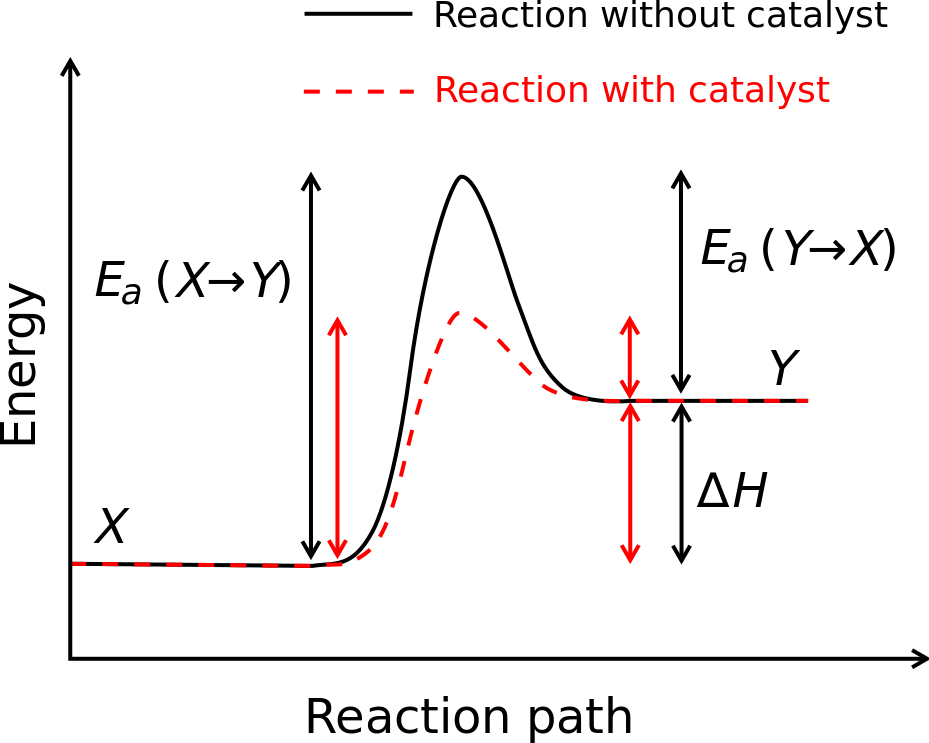
\includegraphics[width=0.7\linewidth]{pictures/Activation_energy} 

}

\caption{Activation Energy *(E~a~)* needed for a reaction to proceed. *(E~a~)* can be lowered thanks to a catalyst, and in the case of the respiration chain of living organisms, many of them. Figure borrowed from Wikipedia, Copyrighted free use, https://commons.wikimedia.org/w/index.php?curid=779552}\label{fig:EnergyActivation}
\end{figure}

In normal conditions, this energy is preventing a reaction to proceed.
This is why wood or most organic matter do not go into combustion or
decomposition on their own. Nitroglycerin is notoriously unstable and
the activation energy for electrons to be transferred to
O\textsubscript{2} is very small, hence its propensity to explode and
its danger. However, the activation energy can be overcome with enough
heat brought near an electron donor in the form of a flame or a spark.
Not much heat is necessary for natural gas (CH\textsubscript{4}) for
combustion to take place, i.e., for transfer of electrons from the
carbon to oxygen, releasing twice the volume of gases:

\begin{equation}
CH_4 + O_2 \Rightarrow CO_2 + H_2O
\label{eq:CH4combustion}
\end{equation}

hence the explosive nature of this reaction.

\section{Generating energy without
combustion}\label{generating-energy-without-combustion}

Now because none of us and all the living organisms with us, \emph{burn}
to generate energy, there must be other systems to manage to liberate
energy, and, there must be ways to have much lower activation energy.
Life has found several mechanisms to optimize the transfer of energy
from organic matter to the a magic molecule:
\protect\hyperlink{ATP}{ATP} or Adenosine TriPhosphate.

\section{ATP or the energy currency of the
cell}\label{atp-or-the-energy-currency-of-the-cell}

There are many ways of transferring energy. To heat a house in the
western world, we most often have a centralized heating (and sometimes
cooling) system, where the heat is generated, e.g., in a furnace, and
then transferred to the rest of the house via pipes and the like. The
equivalent system might be for mammals the blood that gets re-oxygenated
with the lungs, before it delivers oxygen throughout the body.

At the cellular level, however, \protect\hyperlink{ATP}{ATP} or
Adenosine TriPhosphate is created throughout the cell near the
equivalent of the little furnaces: mitochondria. Needless to say, there
is no combustion with the mitochondria, and yet transfer of electrons
and energy delivered. The energy is transferred from the
\protect\hyperlink{OM}{organic matter} to ATP, and ATP being a
relatively small molecule, can easily reach all metabolic processes,
usually operated by proteins, which need energy to proceed (to overcome
the \href{https://en.wikipedia.org/wiki/Activation_energy}{activation
energy} mentioned above).

\begin{figure}

{\centering 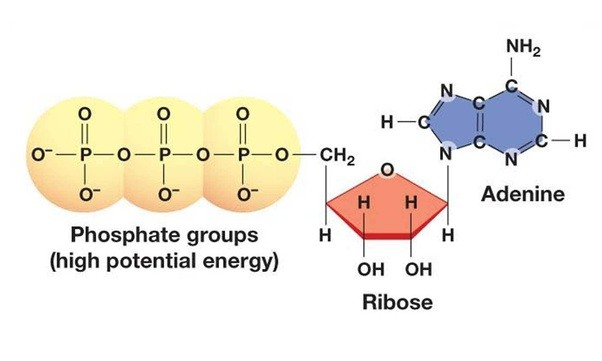
\includegraphics[width=0.7\linewidth]{pictures/atp02a} 

}

\caption{ATP molecular structure containing adenosine (= adenine + ribose) and the three phosphate linked together with a pyrophosphate energy rich bond. Copyrighht Pearson Benjamin Cummings}\label{fig:ATPstructure}
\end{figure}

The key to storing energy is in the bond between the phosphate, which
are often referred to as high-energy bonds. High-energy phosphate bonds
are pyrophosphate bonds, acid anhydride linkages formed by taking
phosphoric acid derivatives and dehydrating them. As a consequence, the
hydrolysis of these bonds is exergonic under physiological conditions,
releasing energy. As ATP releases its energy by the break of the
pyrophosphate bond, ATP thus becomes ADP (Adenosine Diphosphate) and
releases a phosphate in the meantime, like in figure \ref{fig:ATPtoADP}.
A common representation of this reaction is
\(ATP \Rightarrow ADP + P_i\) with the P\textsubscript{i} referring to
as a phosphate.

\begin{figure}

{\centering 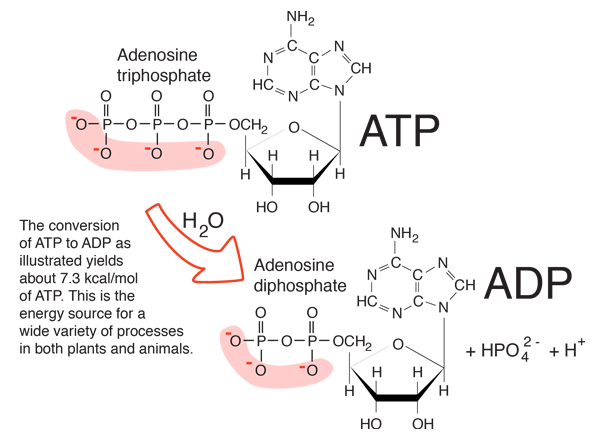
\includegraphics[width=0.8\linewidth]{pictures/atptoadp} 

}

\caption{Release of energy ATP hydrolyzed into ADP. http://hyperphysics.phy-astr.gsu.edu/hbase/Biology/atp.html}\label{fig:ATPtoADP}
\end{figure}

Now that we have allocated electrons on atoms and molecules, you easily
understand that the number of electrons on the outside of the triplet
\(PO_3-O-PO_2-O-PO_2\) is huge. In his fantastic book, Degens
\citeyearpar{Degens1989-ip} suggests that

\begin{itemize}
\tightlist
\item
  because of the plethora of electrons on the triphosphate part of ATP,
\item
  because the tetrahedral phosphate molecules are linked together by one
  of the corners of each tetrahedron (figure \ref{fig:PO4tetrahedra}),
\item
  and because of the \(\pi\) electron bonds (double bond) which tends to
  repulse each other \citep{Degens1989-ip},
\end{itemize}

the triphosphate molecule can only be in constant movement, which
`maintains the animated world' \citep{Degens1989-ip}.

\begin{figure}

{\centering 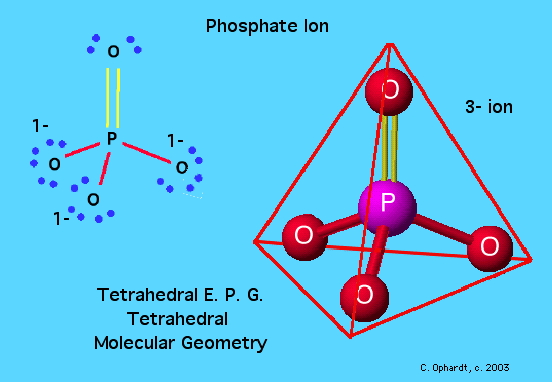
\includegraphics[width=0.6\linewidth]{pictures/204phosphate} 

}

\caption{Tetrahedral configuration of each of the phosphate molecule which when linked together supposedly are in constant movement}\label{fig:PO4tetrahedra}
\end{figure}

\section{The ATP manufacture}\label{the-atp-manufacture}

If ATP freely releases energy for a reaction to proceed in the cell, as
ATP becomes ADP + Pi, there must be energy at one point to `manufacture'
or recharge the ATP molecule in the first place. We have seen that much
of the energy in the cell is transferred thanks to the ATP molecule. So
could we just make ATP from the energy liberated by ATP??? The answer is
no, obviously\ldots{} The energy to create ATP has to come from
elsewhere, otherwise it just cannot work\ldots{}!!!

Life has find a wonderful way to do that thanks to proton flows. Yes,
that is correct, a proton flow. ATP is literally formed from an ADP and
a phosphate and assembled thanks to a protein called ATP synthase, or
ATPase, which seems to be activated or powered almost mechanically, very
much like a water mill, by a proton flow (Figure \ref{fig:ATPase}). You
may want to look at this very nice concise document on
\href{https://en.wikipedia.org/wiki/ATP_synthase}{ATP synthase on
Wikipedia}, which provides more detailed information and shows quite
nicely how the mechanical force of the H\textsuperscript{+} is thought
to allow P\textsubscript{i} to be attached to an ADP. This part of the
energy recovery is referred to as \emph{\textbf{phosphorylation}}.

\begin{figure}

{\centering 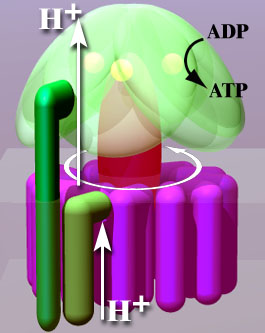
\includegraphics[width=0.4\linewidth]{pictures/Atpsyntase4} 

}

\caption{Artist representation of the ATP synthase powered, almost mechanically by proton flows. By The original uploader was Asw-hamburg at German Wikipedia - Transferred from de.wikipedia to Commons by Leyo using CommonsHelper., CC BY-SA 3.0, https://commons.wikimedia.org/w/index.php?curid=8993938}\label{fig:ATPase}
\end{figure}

So, this mechanical force is what generates the synthesis of ATP from
ADP, or again \emph{\textbf{phosphorylation}}. So this solves that part
of the ATP synthesis. Now, another mechanism must be responsible for the
formation of the proton flow.

\section{Creating a proton gradient as a source of proton
flow}\label{creating-a-proton-gradient-as-a-source-of-proton-flow}

Until now, I have not even mentioned where all this takes place. We are
about to see where this happens. But first, let us take an analogy to
better understand the proton flow responsible for the synthesis of ATP.
Flow of matter just does not happen on its own, it only happens as a
result of a \emph{\textbf{gradient}} between a compartment and another.
Using the water mill analogy, the reason why there is release of energy
in the form of kinetic energy of the water is because there is a drop in
elevation, and therefore in potential energy between the `compartments'
upstream and downstream the mill. To increase the hydraulic gradient,
men throughout the world have built dams to create compartments and
increase the hydraulic gradient between upstream and downstream the
mill. So in the water mill analogy, the hydraulic gradient is maintained
thanks to the dam which creates compartments, and to the continuous
arrival of new water upstream and to the leaving of water downstream. So
three things are necessary for the release of kinetic energy (which in
the end is going to power the rotation of a mill wheel, and in the old
days would grind wheat or corn grain):

\begin{itemize}
\tightlist
\item
  a system to compartmentalize water,
\item
  a supply of water, and,
\item
  an outlet for the water so that is does not accumulate.
\end{itemize}

By analogy, the formation of ATP corresponds to the grain grinding; the
proton flow corresponds to the water flowing that activates the mill
wheel, and in our case the proton flow activates the ATPase. We now need
to address the three parts of the system needed to have a proton
gradient and flow:

\begin{itemize}
\tightlist
\item
  a compartment system,
\item
  a proton supply system, and,
\item
  a system to use protons so the gradient is maintained.
\end{itemize}

\subsection{A compartment to accumulate
protons}\label{a-compartment-to-accumulate-protons}

We saw earlier that the \protect\hyperlink{phospholipids}{double
phospholipid layer} made the cell membrane. Well if you close a membrane
on itself you will make a compartment or a balloon. It turns out that if
you look at a typical prokaryotic cell and at organelles in a eukaryotic
cell (Figure \ref{fig:cells}), there are compartments formed between a
cell wall and the plasma membrane for prokaryotic cells, and between two
double layer phospholipid membranes for the eukaryotic cells. So in
reality, it is a bit as if one were to create a space between two
balloons.

\begin{figure}

{\centering 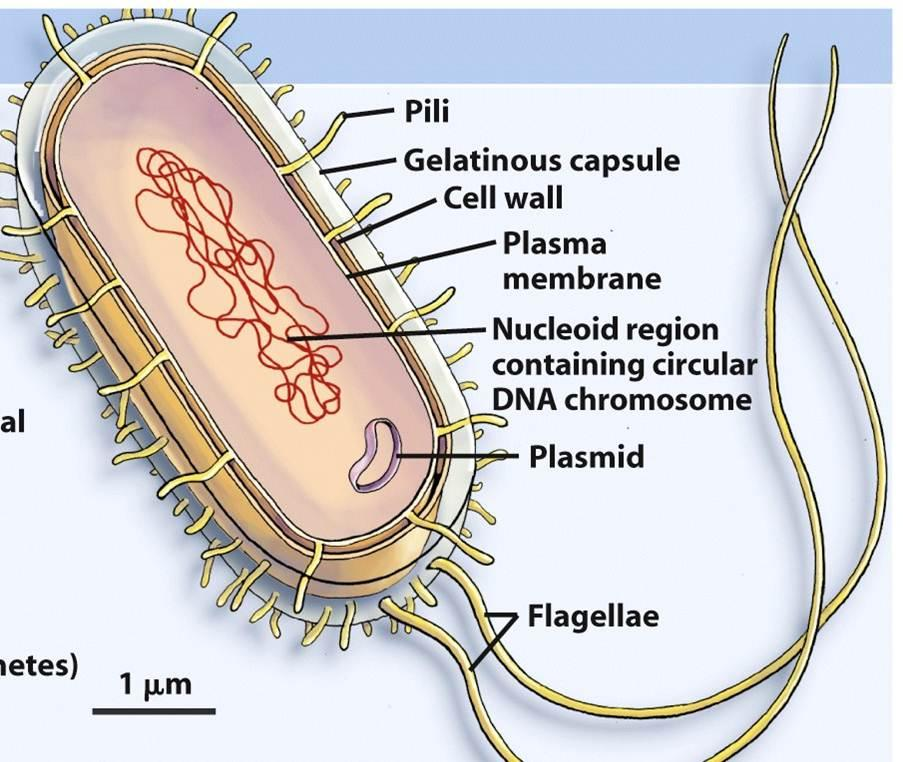
\includegraphics[width=0.45\linewidth]{pictures/prokaryotic-cell-diagram} 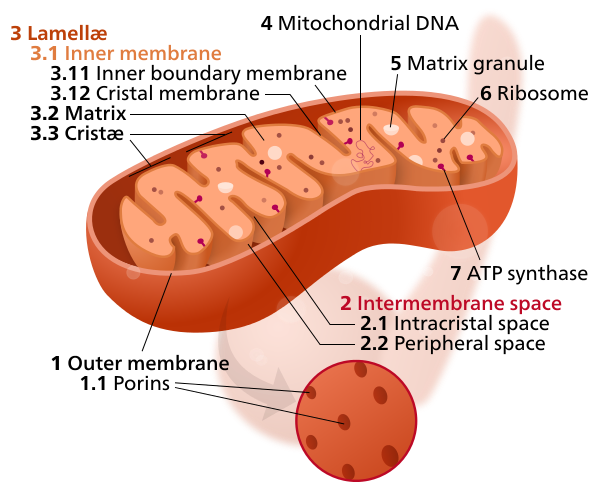
\includegraphics[width=0.45\linewidth]{pictures/Mitochondrion_mini.svg} 

}

\caption{Artist representation of a prokaryotic cell and a mitochondrion from a eukaryotic showing the intermembrane spaces: between the cell wall and plasma membrane for the prokaryotic cell, and, between the outer and inner membranes for the mitochondrion.  https://micro.magnet.fsu.edu/cells/animals/animalmodel.html and By Kelvinsong - Own work, CC0, https://commons.wikimedia.org/w/index.php?curid=27715320}\label{fig:cells}
\end{figure}

At the end though, there exists for prokaryotic cells and mitochondria
(and most organelles for eukaryotic cell) an inter-membrane space, which
effectively creates compartments to accumulate `things'. The double
phospholipid membrane is so strong and so tight that it is
\emph{proton-tight}. In other words, if somehow protons accumulate in
this inter-membrane space, protons cannot leave through the membrane,
they can only leave through designated areas. And yes, you guessed
right, the designated area for protons to leave the inter-membrane space
is the ATP synthase! So to take another analogy, you can imagine an
inner tube full of air under pressure, air can only leave through the
valve. And if you were to put a little fan in front of the valve as you
are releasing air, the fan would rotate. Imagine that this is
essentially what happens: the ATPase is both the valve and the fan as it
\href{https://upload.wikimedia.org/wikipedia/commons/6/62/ATPsyn.gif}{literally
rotates with the proton flow}.

\subsection{A supply of protons for the intermembrane space: proton
pumps}\label{a-supply-of-protons-for-the-intermembrane-space-proton-pumps}

Now, the next natural question is that in the case of an inner tube,
somebody pumped some air into the tube to put it under pressure.
Similarly, there must be a system that pumps protons into the
inter-membrane space. And yes indeed, you guessed it right, there are
proton pumps that do the job. But again, these pumps must be powered by
some sort of energy.

Let us pause for a second. We have seen in section
\ref{generating-energy-transfer-of-electrons} that generally speaking,
energy is generated from the transfer of electrons. But until now, we
have not even mentioned electrons: only ATP and protons\ldots{}? This is
where electrons come in: \textbf{energetic electrons transported onto
electron transfer molecules are the ones that power the proton pumps!}.
It is time to take a bird's eye view again. Energy liberation exists
when electrons are transferred from an electron donor to an electron
acceptor. Life has found a way to capture this energy in the form of
ATP, which allows transportation of energy to the needed places in the
cell. So the energy transfer in the cell does not have to be totally
instantaneous like combustion would be, and it can be spent exactly
where it needs to be spent.

Yet, the production of ATP is in fact generated by an electron transfer,
but indirectly.

\begin{itemize}
\tightlist
\item
  No, electrons are \textbf{NOT} transferred from organic matter to ATP.
\item
  Yes, electrons are \emph{ultimately} transferred from organic matter
  to an electron acceptor, which in the case of aerobic respiration is
  O\textsubscript{2}.
\end{itemize}

But just like the generation of ATP is indirectly linked to the electron
transfer, the transfer of electrons from organic matter to the ultimate
electron acceptor is also indirect. A set of molecules called
\textbf{electron transfer molecules} are intermediate carrier of
electrons and are the ones which power the proton pumps as represented
in figure \ref{fig:protonpumps} below.

\begin{figure}

{\centering 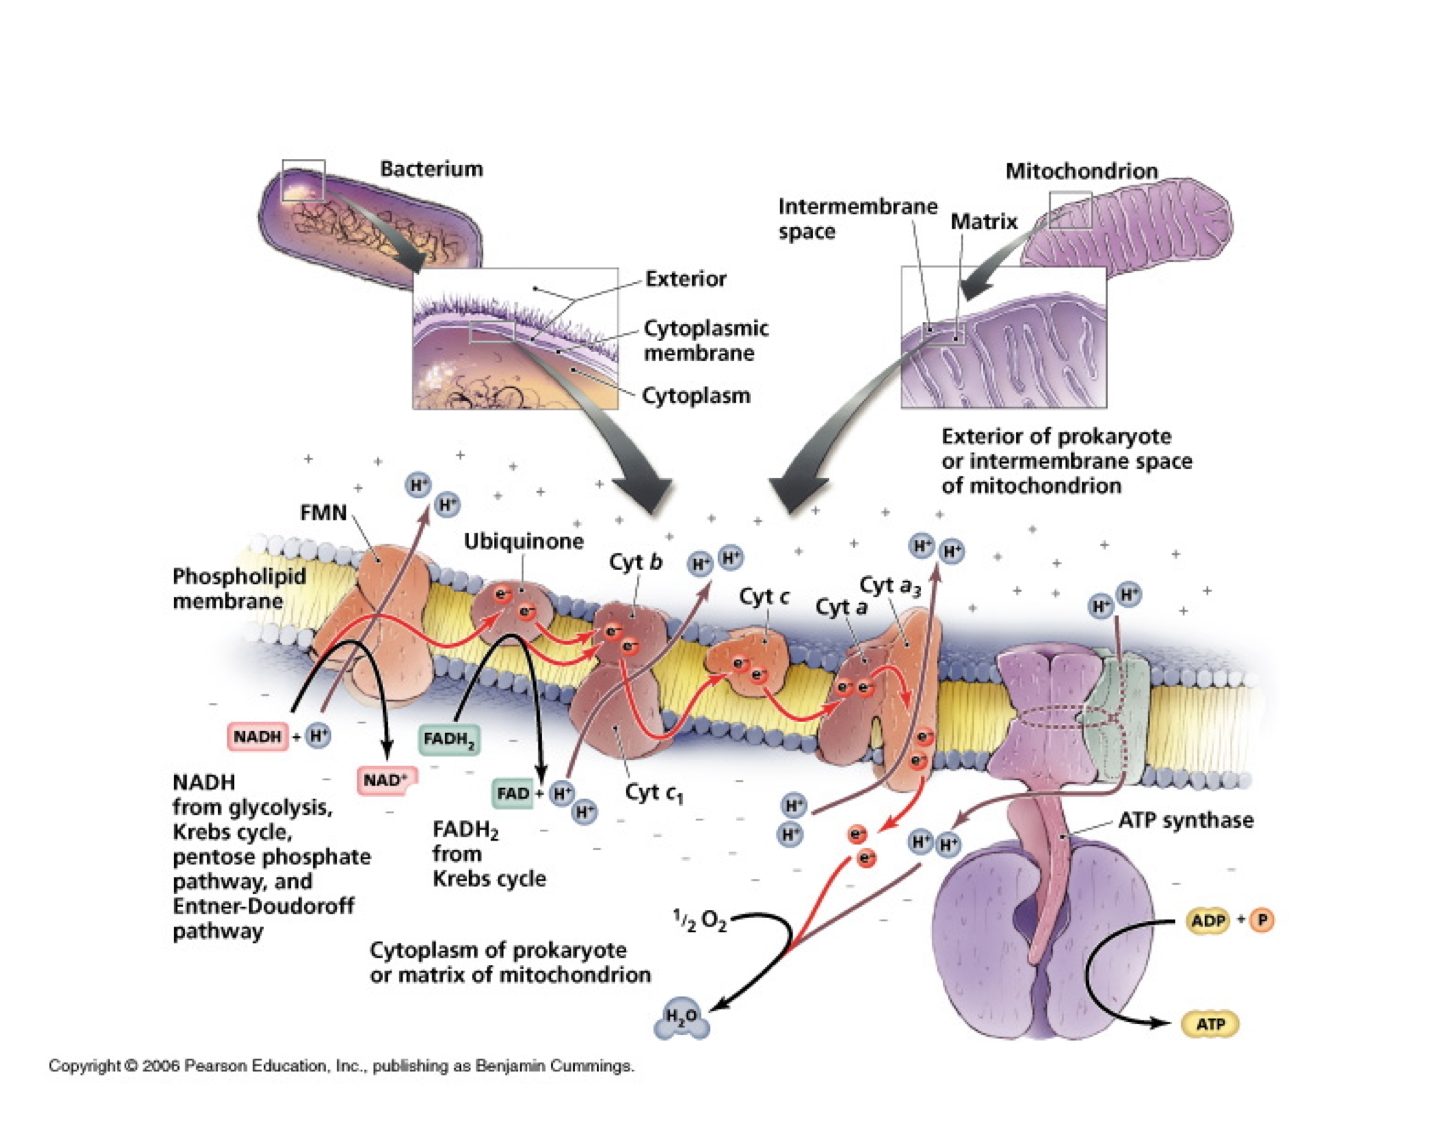
\includegraphics[width=1\linewidth]{pictures/membrane_proton_pumps} 

}

\caption{Artist representation of the ATP synthesis powered by a proton flow, itself powered by a proton gradient, itself produced thanks to proton pumps powered by energy rich electrons carried by electron transfer molecules. Obtained from 2006 Pearson Education}\label{fig:protonpumps}
\end{figure}

\hypertarget{electron-transfer-molecules-that-power-the-proton-pumps}{\subsection{Electron
transfer molecules that power the proton
pumps}\label{electron-transfer-molecules-that-power-the-proton-pumps}}

The two main electron transfer molecules in the respiration process are
called NAD (Nicotinamide Adenine Dinucleotide; figure \ref{fig:NAD}) and
FAD (flavine adenine dinucleotide; figure \ref{fig:FAD}). These two
nucleotides have the ability to be reduced (= gain electrons) and
oxidized (= lose electrons), and because they are mobile, to carry
electrons from the cell (bacteria) or mitochondrion (eukaryot) cytoplasm
to the proton pumps.

\begin{figure}

{\centering 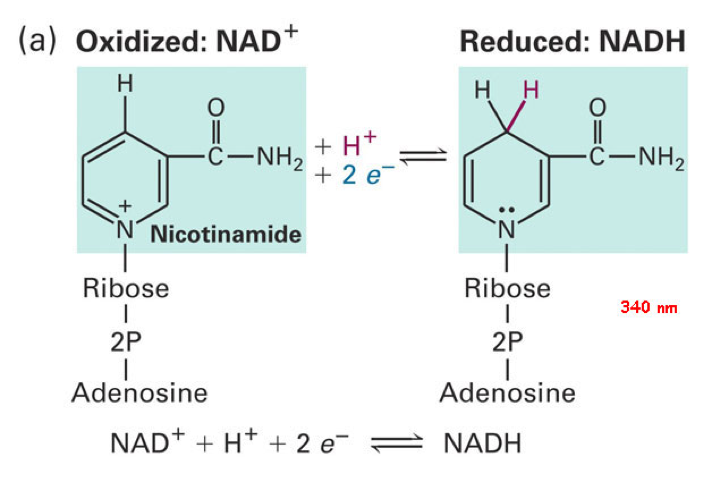
\includegraphics[width=0.45\linewidth]{pictures/NADreduction} 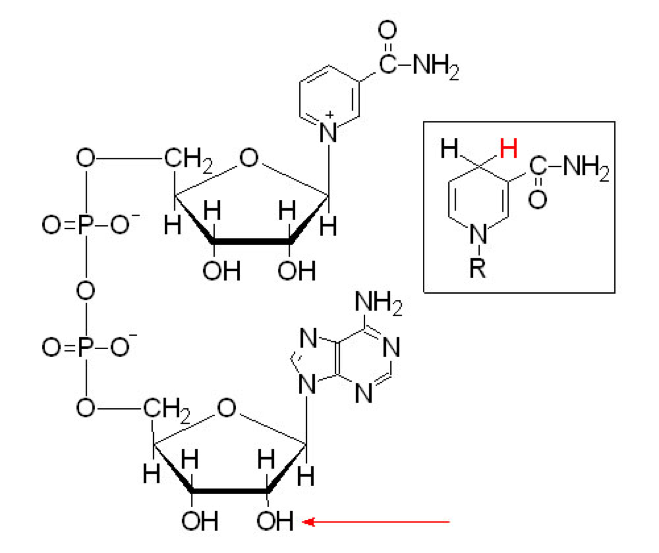
\includegraphics[width=0.45\linewidth]{pictures/NADfull} 

}

\caption{Molecular formula of Nicotinamide Adenine Dinucleotide (NAD) in both oxydized and reduced states}\label{fig:NAD}
\end{figure}

\begin{figure}

{\centering 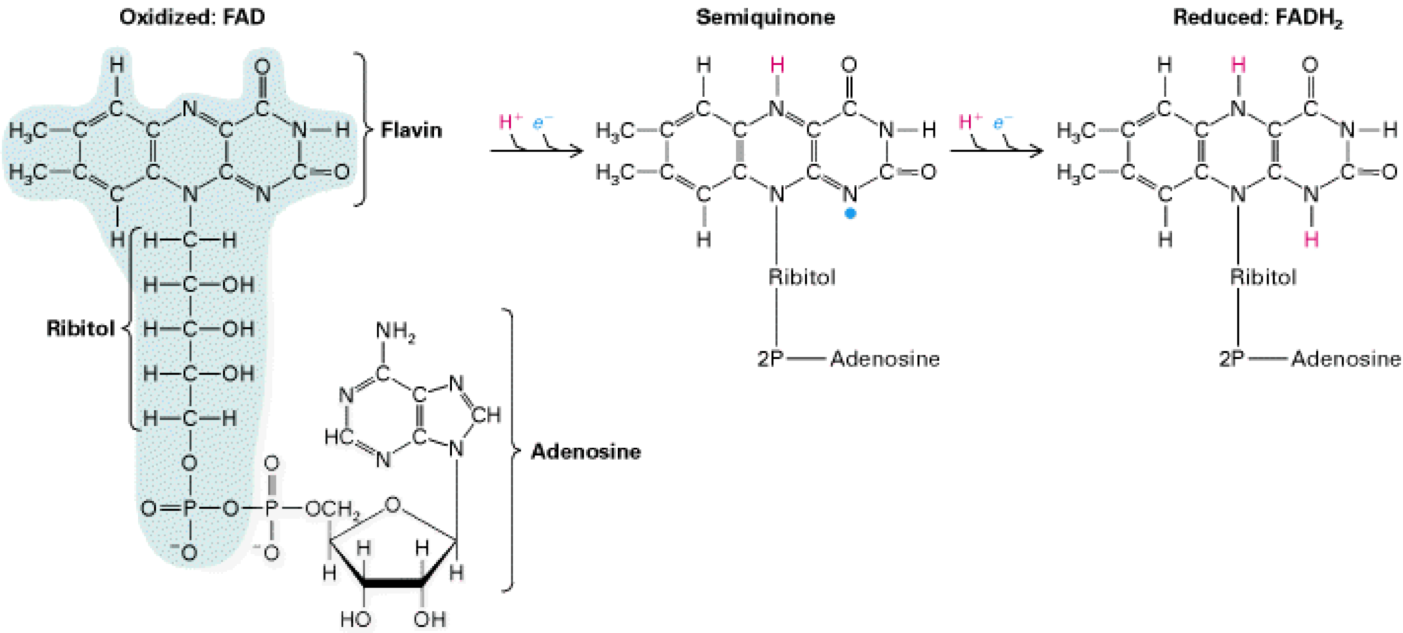
\includegraphics[width=1\linewidth]{pictures/FAD} 

}

\caption{Molecular formula of Flavine Adenine Dinucleotide (FAD) in both oxydized and reduced states}\label{fig:FAD}
\end{figure}

\section{Transfer of electrons from the Organic Carbon to an electron
acceptor}\label{transfer-of-electrons-from-the-organic-carbon-to-an-electron-acceptor}

So this answers the question of how the proton pumps are powered, but it
is now time to look at the global fate of electrons: where do they come
from and where do they end up? Actually, we already know the global
answers to these questions: the electrons are stored unto the C, N, and
S of organic molecules and they are eventually accepted by an electron
acceptor; in the case of aerobic respiration, O\textsubscript{2} is the
ultimate electron acceptor.

Before there might be any confusion, in the aerobic respiration process
that involves organic molecules as electron donors (we will see that
inorganic molecules can also be electron donors), strangely enough, the
only atom which donates electron is \textbf{carbon} while the nitrogen
and sulfur atoms keep all their eight electrons. Specialized microbes,
called \emph{\protect\hyperlink{lithotrophs}{lithotrophs}}, literally
`feed on stone', which means that their source of electron is from an
inorganic molecule, have the ability to use ammonium and hydrogen
sulfide as electron donor (8 electrons available for `donation') in
their aerobic respiration chains. So all this to say that in aerobic
respiration that involves organic matter, \textbf{only} the carbon atom
donates its electrons. The organisms which use organic matter as
electron donors are called \emph{organotrophs}. We, as mamals and
humans, are \emph{organotrophs}.

\subsection{Oxygen reduction}\label{oxygen-reduction}

Let us start from the end of the process: the reduction of oxygen into
H\textsubscript{2}O, as represented on figure \ref{fig:protonpumps}
above. As the NAD and FAD are powering proton pumps (which names include
FMN, ubiquinone, cytochrome a, b, and c see figure
\ref{fig:protonpumps}), the electrons lose some of their energy and
migrate within the phospholipid membrane from the proton pumps towards
the ATPase. Because of the involvment of many different proteins
involved in this transport, this is referred to as the
\emph{\textbf{electron transfer chain}}. Because the NAD and the FAD
molecules are oxidized (they have given up their electrons), and because
at the ATPase location, ADP gains a phosphate to become ATP, the whole
process is referred to as \emph{\textbf{oxidative phosphorylation}}. At
the confluence between the ATPase and the cytochrome a\textsubscript{3},
the reaction \eqref{eq:O2reduction} occurs:

\begin{equation}
O_2 + 4 e^- + 4 H^+ \Rightarrow 2 H_2O
\label{eq:O2reduction}
\end{equation}

This is the place where the electrons are accepted!!! So now you know
exactly where all this is happening! Is not that wonderful? So the
electrons are accepted by O\textsubscript{2} (remember on a molecule of
O\textsubscript{2}, each Oxygen atom only has 6 electrons for itself, so
each can accept two more), and these electrons reduce oxygen into
H\textsubscript{2}O. This has several consequences:

\begin{itemize}
\tightlist
\item
  the reduction of O\textsubscript{2} also consumes 4
  H\textsuperscript{+}, which solves the necessity for an outlet for
  protons as they flow out of the inter-membrane through the ATPase,
  which was the third condition to maintain a proton gradient
\item
  the reduction of O\textsubscript{2} obviously consumes electrons,
  which also provides an outlet for the electrons. In order words, if no
  electron acceptors are available, then the electrons at the proton
  pumps have no outlet, so the proton pumps are stalled, which in turn
  halts the maintaining of a proton gradient, which eventually stops the
  production of ATP.
\end{itemize}

\subsection{Electron fate from organic matter to electron transfer
molecules}\label{electron-fate-from-organic-matter-to-electron-transfer-molecules}

The fate of electrons from organic matter or glucose to the electron
transfer molecules involves two processes called
\protect\hyperlink{glycolysis}{glycolysis} and the
\protect\hyperlink{krebscycle}{Krebs or citric acid cycle}. Biology
majors have to learn in details all the steps and the name of the
molecules involved in these chain reactions. This is beside our point
for our class. Instead I want you to understand and know that these
reactions involve

\begin{itemize}
\tightlist
\item
  transfer of electrons from organic carbon onto
  \protect\hyperlink{electron-transfer-molecules-that-power-the-proton-pumps}{electron
  transfer molecules}
\item
  the release of carbon atoms which have lost all their electrons,
  therefore releasing C in the form of CO\textsubscript{2}.
\item
  the hydrolysis of glucose molecules to
  \href{https://en.wikipedia.org/wiki/Pyruvic_acid}{pyruvate}, a C3
  molecule (a 3 carbon organic molecule) during the glycolysis, which
  then loses CO\textsubscript{2} as it enters the citric cycle
\item
  the acetyl-coA, a co-enzyme is key to incorporate organic carbon in
  the Krebs cycle.
\end{itemize}

In figure \ref{fig:respirationglobal} below which summarizes all the
aerobic respiration pathways, you can see that most of the ATP is formed
thanks to the proton flow, and that
\protect\hyperlink{electron-transfer-molecules-that-power-the-proton-pumps}{electron
transfer molecules} are involved in all steps.

\begin{figure}

{\centering 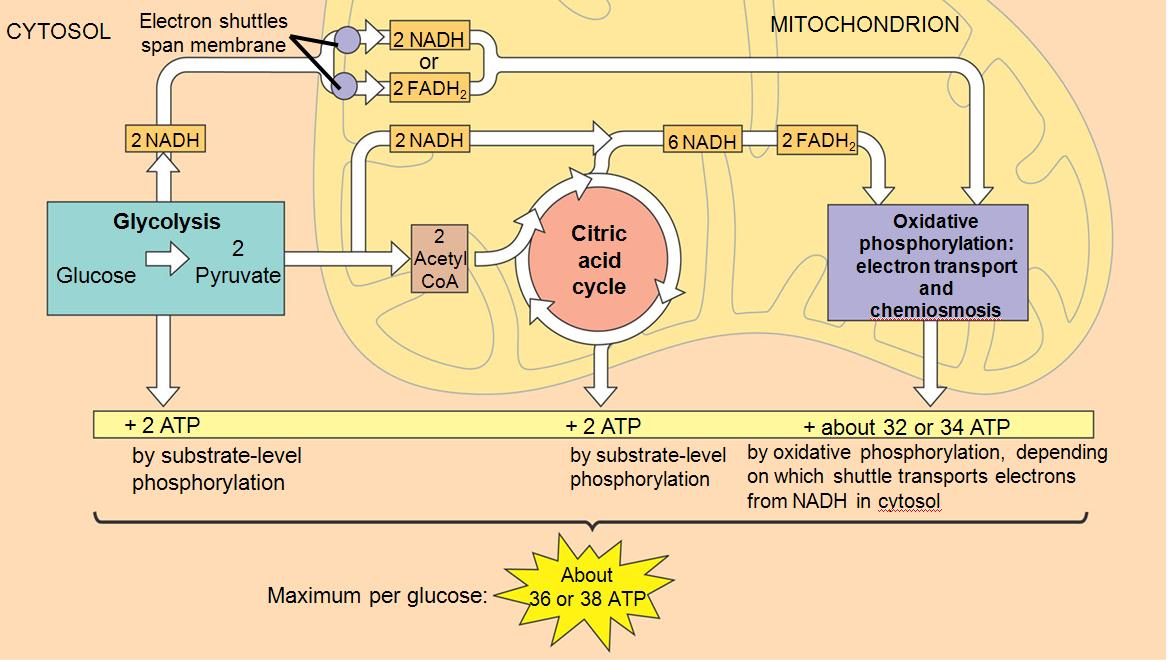
\includegraphics[width=0.95\linewidth]{pictures/respiration_global} 

}

\caption{Summary of cellular respiration with the ATP and electron transfer budget. Obtained from https://cdn.thinglink.me/api/image/847806852426104839/1240/10/scaletowidth}\label{fig:respirationglobal}
\end{figure}

This \ref{fig:respirationglobal} diagram does not show where the
CO\textsubscript{2} are produced so I invite to see, in addition to the
notes given in class, that CO\textsubscript{2} is released as pyruvic
acid enters in the figures \ref{fig:krebs} and \ref{fig:glycolysis}
below.

\begin{figure}

{\centering 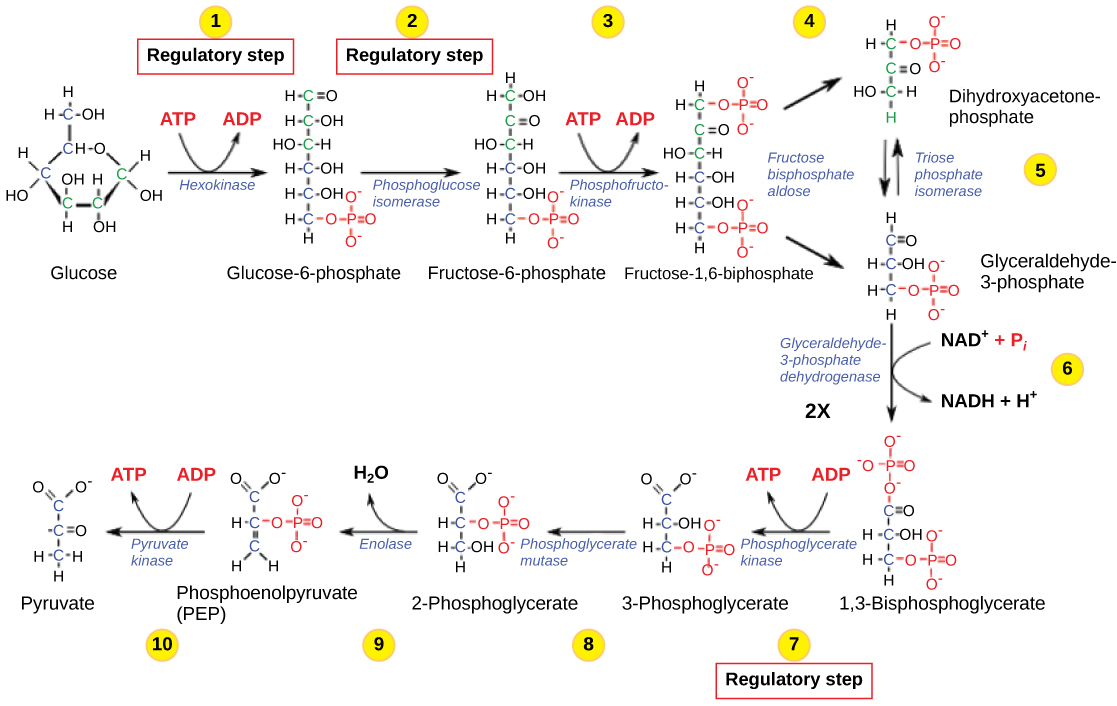
\includegraphics[width=0.95\linewidth]{pictures/Glycolysis} 

}

\caption{Glycolysis pathway. Image}\label{fig:glycolysis}
\end{figure}

\begin{figure}

{\centering 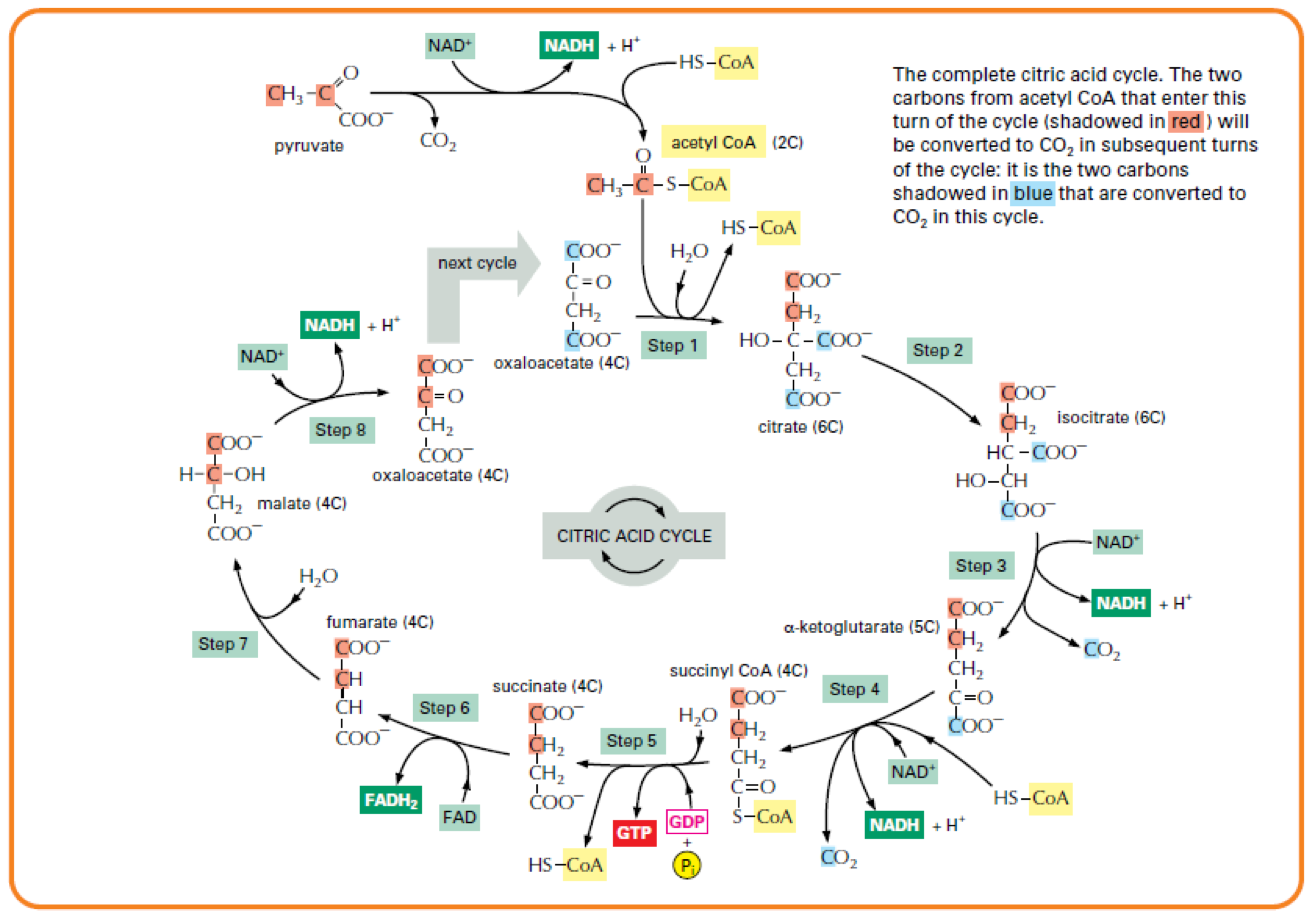
\includegraphics[width=0.95\linewidth]{pictures/Krebscycle} 

}

\caption{Krebs or citric acid cycle pathway.}\label{fig:krebs}
\end{figure}

\section{Summary of respiration}\label{summary-of-respiration}

We have purposely presented the molecular processes of respiration
starting from the end and moving back to the beginning of the
respiration chain. We can summarize the respiration process again in
that order:

\begin{itemize}
\tightlist
\item
  the goal of respiration is to transfer energy initially stored as high
  energy electrons on organic molecules to ATP, the energy currency of
  the cell
\item
  The production of ATP itself has to come from a different source of
  energy than that liberated by ATP itself
\item
  ATP is synthesized by the phosphorylation of ADP by the ATP synthase,
  itself powered by a proton flow from the inter-membrane space to the
  cytoplasm space
\item
  the proton flow is powered by a proton gradient between the
  inter-membrane space and the cytoplasm space
\item
  This gradient is made possible thanks to

  \begin{itemize}
  \tightlist
  \item
    a proton-tight compartment corresponding to the inter-membrane space
  \item
    a supply of protons from the cytoplasm to the inter-membrane space,
    fed by proton pumps
  \item
    an outlet for the protons flowing out and powering the ATPase (`the
    proton mill'), which combined with the reduction of oxygen form
    water molecules
  \end{itemize}
\item
  The proton pumps are themselves powered by the oxidation of electron
  transfer molecules (NAD and FAD), which carry high energy electrons
  from the Krebs or citric cycle to the electron transfer chain
\item
  The electron transfer molecules accept the electrons, or are reduced
  during glycolysis, before and during the Krebs cycle as organic carbon
  are oxidized or lose their electrons and release CO\textsubscript{2}.
\end{itemize}

The other way to present respiration is to say that:

\begin{itemize}
\tightlist
\item
  Energy rich electrons stored on organic molecules are transferred onto
  electron transfer molecules during glycolysis, before and during the
  Krebs cycle
\item
  The high energy electrons thus transported power proton pumps placed
  in the inner membrane of the cell for unicellular organisms or of the
  mitochodrion for eukaryotic cells
\item
  These pumps feed a supply of protons to the inter-membrane space
  which, because this space is proton-tight, and because protons outlets
  are limited to the ATP synthase, creates an accumulation of protons in
  this space
\item
  The accumulation of protons creates a proton gradient between the
  inter-membrane space and the cytoplasm, which generates a proton flow
  at designated `holes' in the membrane
\item
  The protons flow out the inter-membrane through the ATP synthase which
  can be approximated by proton canals and almost mechanically turn the
  ATPase head which acts as a `proton mill'
\item
  This proton mill catalyzes the phosphorylation of ADP into ATP
\item
  The proton gradient is maintained possible because the protons flowing
  out of the inter-membrane space are combined with electrons reducing
  oxygen into water
\item
  The electron flow is maintained thanks to the same oxygen reduction,
  which in turns allows electron transfer molecules to be oxidized so
  that then can take their `proton load' again.
\item
  Overall respiration consists in transferring high energy electrons
  from organic molecules to oxygen, and by doing so creating a proton
  gradient which in turn is the main driver for the formation of ATP in
  the cell.
\end{itemize}

Both summaries present the same story but have their own logic. Other
important subtleties of respiration include:

\begin{itemize}
\tightlist
\item
  In the case organic molecules are the source of electrons, only the
  carbon atom donates electrons, the amino and thiol radicals being
  eliminated as a by-product DO NOT donate their electrons in this
  respiration system. This is admitedly a bit weird as the the amino and
  thiol groups still have 8 electrons to donate each.
\end{itemize}

\section{Respiration electron flow
schemes}\label{respiration-electron-flow-schemes}

\chapter{BAE 204 Glossary}\label{bae-204-glossary}

This glossary is meant to assemble terms that we routinely use in
Environmental Sciences and Engineering and which are expected to be
mastered by students taking BAE 204 at NC State university. They are
ordered in alphabetical list for better retrieval and look up.

\section{A}\label{a}

\subsection{Aerobic respiration}\label{aerobic-respiration}

\subsection{Anaerobic respiration}\label{anaerobic-respiration}

\subsection{Ammonia}\label{ammonia}

\begin{itemize}
\tightlist
\item
  \href{https://en.wikipedia.org/wiki/Ammonia}{Ammonia} is a colorless
  gas with a characteristic pungent smell
\item
  Formula: \(NH_3\)
\item
  Ammonia 3D shape:
  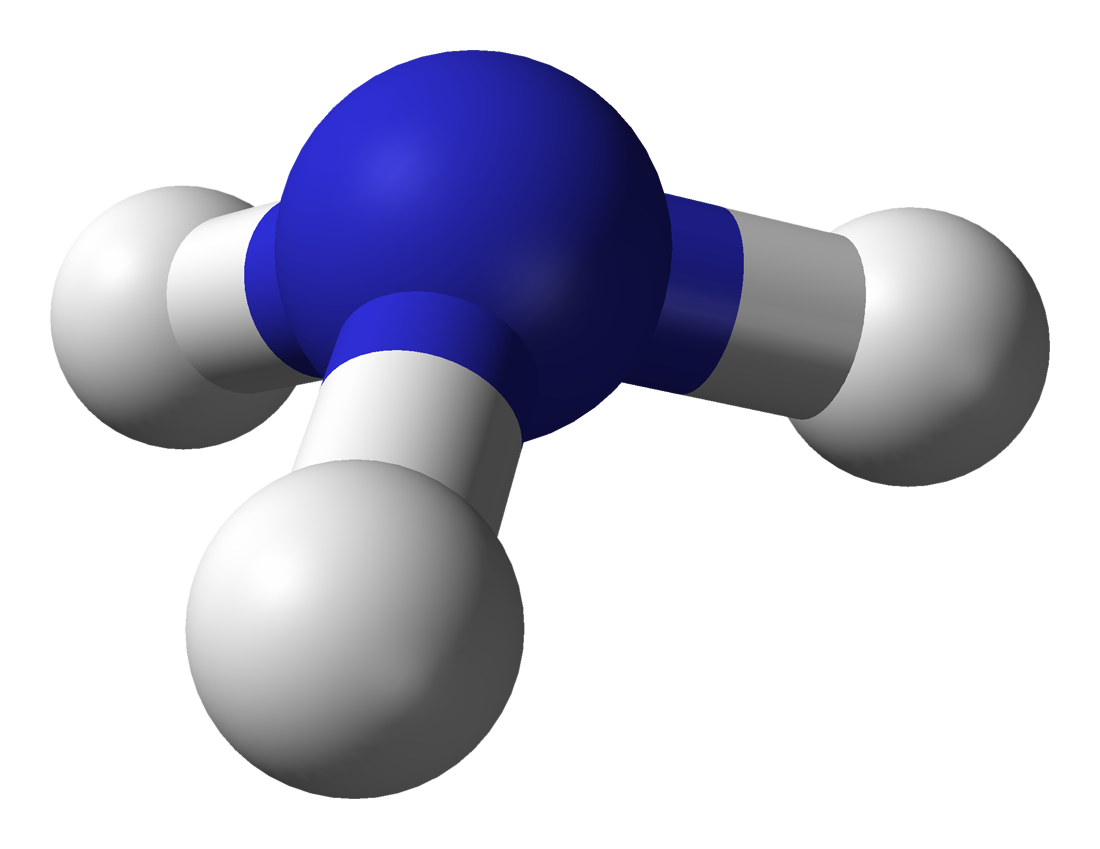
\includegraphics[width=0.25000\textwidth]{pictures/Ammonia-3D-balls-A.png}
\item
  Lewis dot structure:
  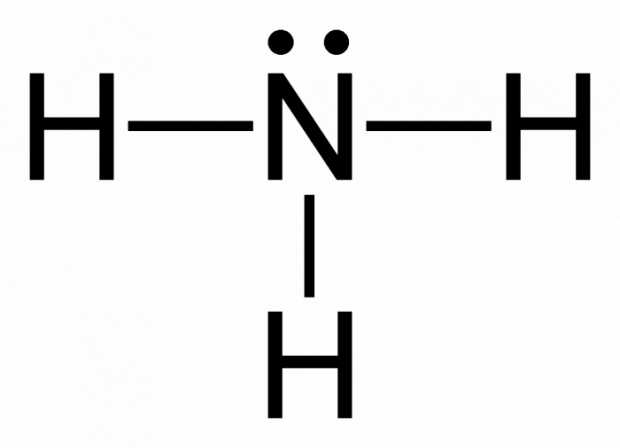
\includegraphics[width=0.25000\textwidth]{pictures/ammonia-lewis-structure.jpg}
\item
  Number of electron N has for itself following electronegativity rule:
  eight
\item
  \(NH_3\) can only be an \textbf{electron donor}
\item
  Because N has so many electrons to be potentially donated, ammonia is
  generally unstable in an aerobic environment. As a result, it tends to
  trace quantities in nature
\item
  When dissolved in water, and depending on the pH of the solution,
  ammonia converts to \protect\hyperlink{NH4}{ammonium} following the
  reaction:
\end{itemize}

\[
H_2O + NH_3 \rightleftharpoons OH^{-} + NH_4^{+}
\]

\begin{itemize}
\tightlist
\item
  Production:

  \begin{itemize}
  \item
    Because of its many uses, ammonia is one of the most highly produced
    inorganic chemicals. Dozens of chemical plants worldwide produce
    ammonia. Consuming more than 1\% of all man-made power, ammonia
    production is a significant component of the world energy budget.
  \item
    In 2014, about 88\% of the ammonia produced was used for fertilizing
    agricultural crops
  \item
    Modern ammonia-producing plants generally depend on the
    \protect\hyperlink{haber-bosch}{Haber-Bosch process} which consists
    into reducing dinitrogen into ammonia

    \[
    3\,H_2 + N_2 \to 2\,NH_3
    \]
  \end{itemize}
\item
  Consumption:

  \begin{itemize}
  \item
    Ammonia is directly or indirectly the precursor to most
    nitrogen-containing compounds. Virtually all synthetic nitrogen
    compounds are derived from ammonia.
  \item
  \end{itemize}
\end{itemize}

\emph{\protect\hyperlink{top}{back to top}}

\subsection{Ammonium}\label{ammonium}

\begin{itemize}
\tightlist
\item
  \href{https://en.wikipedia.org/wiki/Ammonium}{Ammonium} is the most
  reduced inorganic nitrogenous cation (positively charged).
\item
  Ammonium 3D shape:
  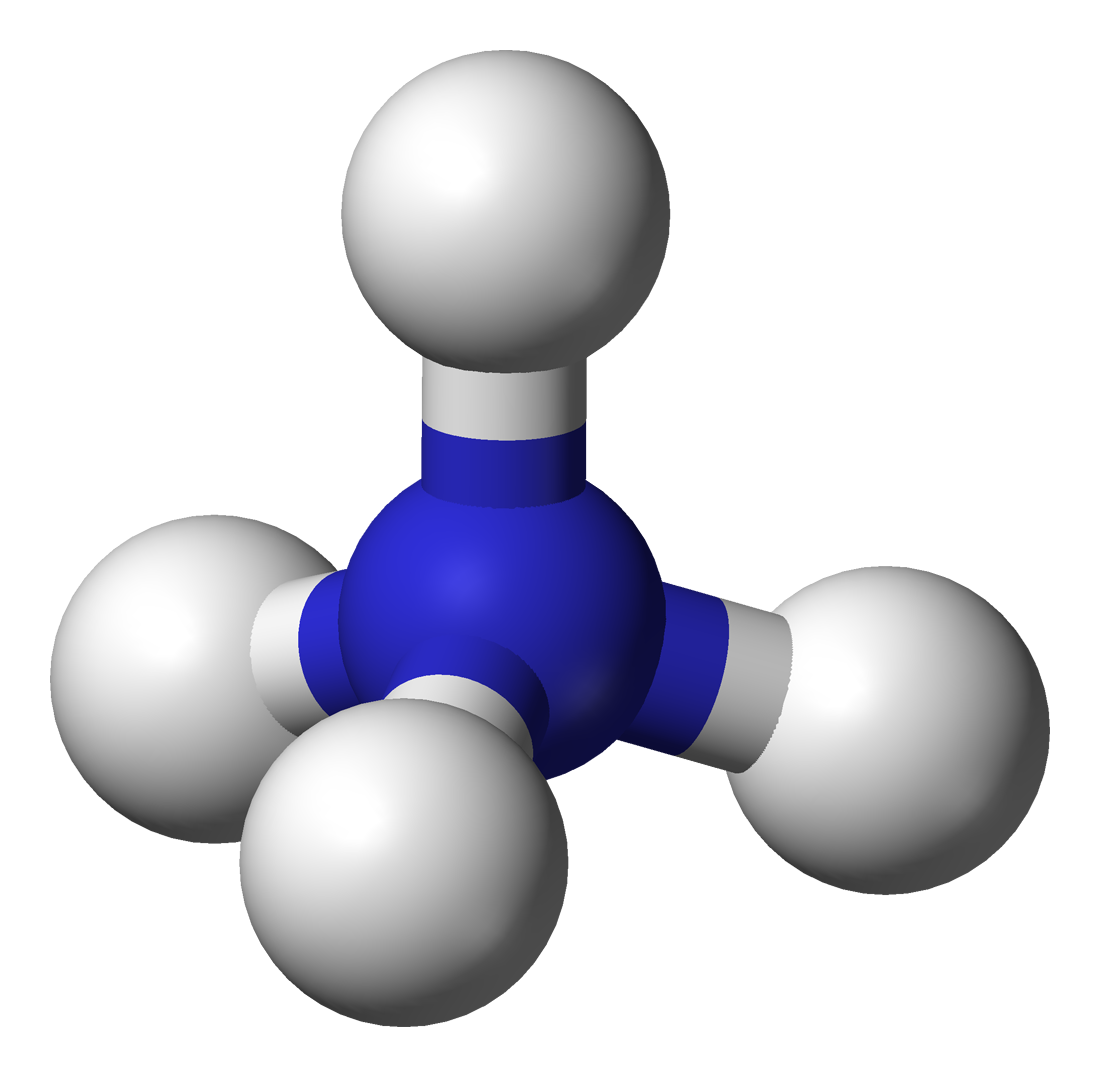
\includegraphics[width=0.25000\textwidth]{pictures/Ammonium-3D-balls.png}
\item
  Lewis dot structure:
  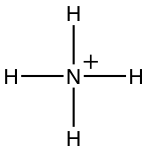
\includegraphics[width=0.25000\textwidth]{pictures/ammonium_lewis_structure.png}
\item
  Number of electron N has for itself following electronegativity rule:
  eight
\item
  It is formed by the protonation of \protect\hyperlink{NH3}{ammonia}
  following the reaction:
\end{itemize}

\begin{equation}
H_2O + NH_3 \rightleftharpoons OH^{-} + NH_4^{+} \label{eq:NH3}
\end{equation}

\begin{itemize}
\tightlist
\item
  The relative abundance of ammonium vs ammonia depends on the pH of the
  solution. See figure below
\end{itemize}

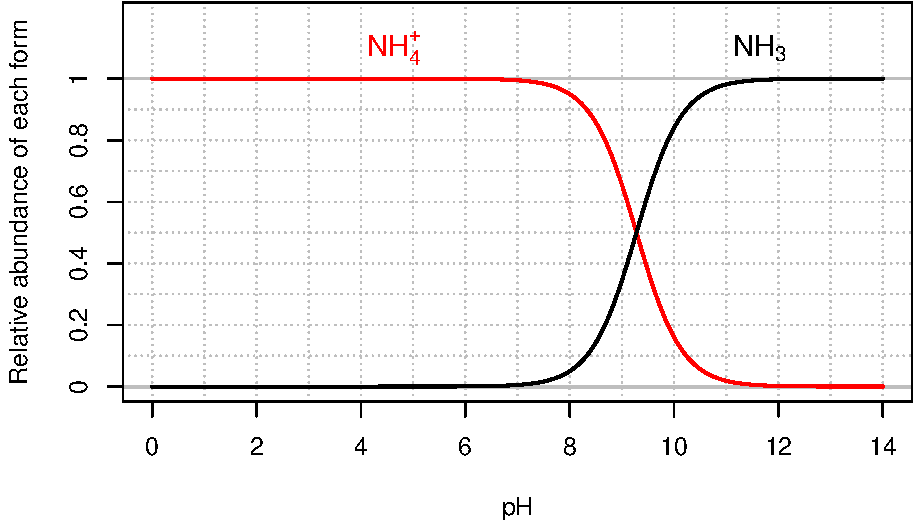
\includegraphics{bookdown-demo_files/figure-latex/NH3-NH4-1.pdf}

\begin{itemize}
\tightlist
\item
  Because in most natural aqueous environments, pH is below 8, ammonium
  tends to be the preponderant form.
\item
  Production:

  \begin{itemize}
  \tightlist
  \item
    In nature, ammonium is a waste product of the mineralization of
    organic molecules
  \item
    It is added as fertilizer on soils as
    \href{https://en.wikipedia.org/wiki/Ammonium_nitrate}{ammonium
    nitrate}
  \end{itemize}
\item
  Health hazard:

  \begin{itemize}
  \tightlist
  \item
    Ammonia vapor has a sharp, irritating, pungent odor that acts as a
    warning of potentially dangerous exposure
  \item
    Exposure to very high concentrations of gaseous ammonia can result
    in lung damage and death
  \end{itemize}
\item
  Drinking water standard:
\end{itemize}

\emph{\protect\hyperlink{top}{back to top}}

\subsection{Ammonium nitrate}\label{ammonium-nitrate}

\begin{itemize}
\item
  \href{https://en.wikipedia.org/wiki/Ammonium_nitrate}{Ammonium
  nitrate} is a chemical compound, the nitrate salt of the ammonium
  cation
\item
  It is a white crystal solid and is highly soluble in water.
\item
  Formula: \(NH_4NO_3\)
\item
  3D shape:
  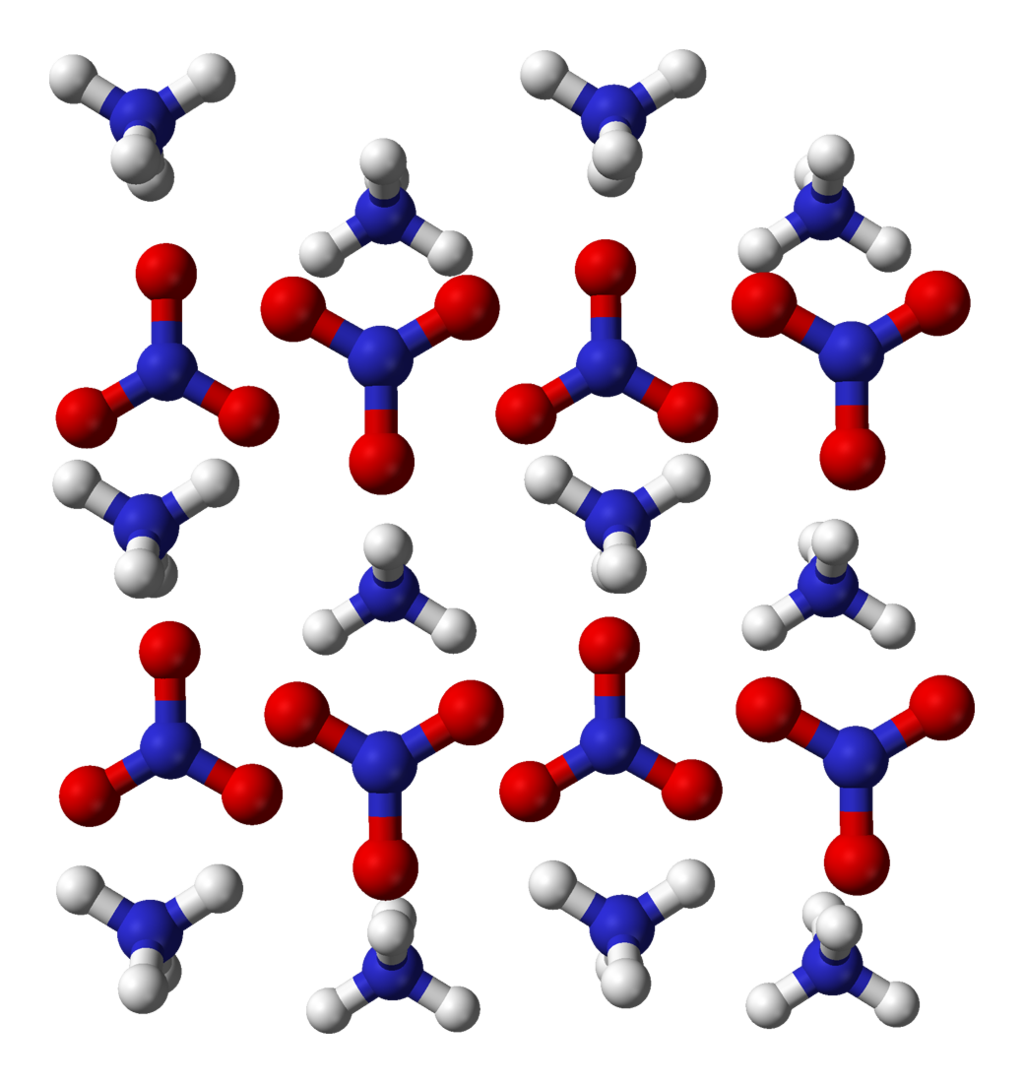
\includegraphics[width=0.33000\textwidth]{pictures/Ammonium-nitrate-xtal-3D-balls-A.png}
\item
  It is predominantly used in agriculture as a high-nitrogen fertilizer
\item
  Its other major use is as a component of explosive mixtures used in
  mining, quarrying, and civil construction
\item
  Production:

  \begin{itemize}
  \tightlist
  \item
    Ammonium nitrate does exist naturally in mines of the
    \href{https://en.wikipedia.org/wiki/Atacama_Desert}{Atacama desert}
    in Chile but globally nearly all ammonium nitrate is now produced
    synthetically
  \item
    Byproduct of all respiration processes. Ammonium ions are a waste
    product of the metabolism of animals. In fish and aquatic
    invertebrates, it is excreted directly into the water. In mammals,
    sharks, and amphibians, it is converted in the urea cycle to urea,
    because urea is less toxic and can be stored more efficiently. In
    birds, reptiles, and terrestrial snails, metabolic ammonium is
    converted into uric acid, which is solid and can therefore be
    excreted with minimal water loss.
  \end{itemize}
\item
  Consumption/utilization:

  \begin{itemize}
  \tightlist
  \item
    It is used as a fertilizer, because it tends to release inorganic
    nitrogen slowly in soil. Applied as a surface fertilizer, it
    penetrates the soil with rainfall infiltration. Highly soluble, the
    nitrate anion becomes readily available to plant roots, although it
    is susceptible to leaching below the root system into the shallow
    and deep groundwater. The ammonium cation tends to adsorb to soil
    particles and is thus not as susceptible to leaching. Ammonium can
    be directly uptaken by plant roots, which thermodynamically makes
    sense, although because in most soils aerobic conditions are
    preponderant, nitrate tends to be the ion uptaken most often. Soil
    bacteria in the aerobic zone of the soil will oxidize adsorbed
    ammonium into nitrate, which then becomes available for plant roots.
    The whole chain of events slows the release of inorganic nitrogen to
    crops and thus makes for more effective fertilizers.
  \end{itemize}
\item
  Health hazard

  \begin{itemize}
  \tightlist
  \item
    No direct known health hazard
  \end{itemize}
\end{itemize}

\emph{\protect\hyperlink{top}{back to top}}

\subsection{Anoxic waters}\label{anoxic-waters}

\begin{itemize}
\tightlist
\item
  Anoxic waters are areas of sea water, fresh water, or groundwater that
  are depleted of dissolved oxygen and are a more severe condition of
  hypoxia (Wikipedia)
\item
  Anoxic waters result from an \emph{\textbf{IMBALANCE}} between oxygen
  supply and demand
\end{itemize}

\emph{\protect\hyperlink{top}{back to top}}

\section{C}\label{c}

\subsection{Carbon dioxide}\label{carbon-dioxide}

\begin{itemize}
\item
  Carbon dioxide is a colorless gas which density is 50\% higher than
  that of dry air.
\item
  Formula: \(CO_2\)
\item
  Carbon dioxide 3D shape:
  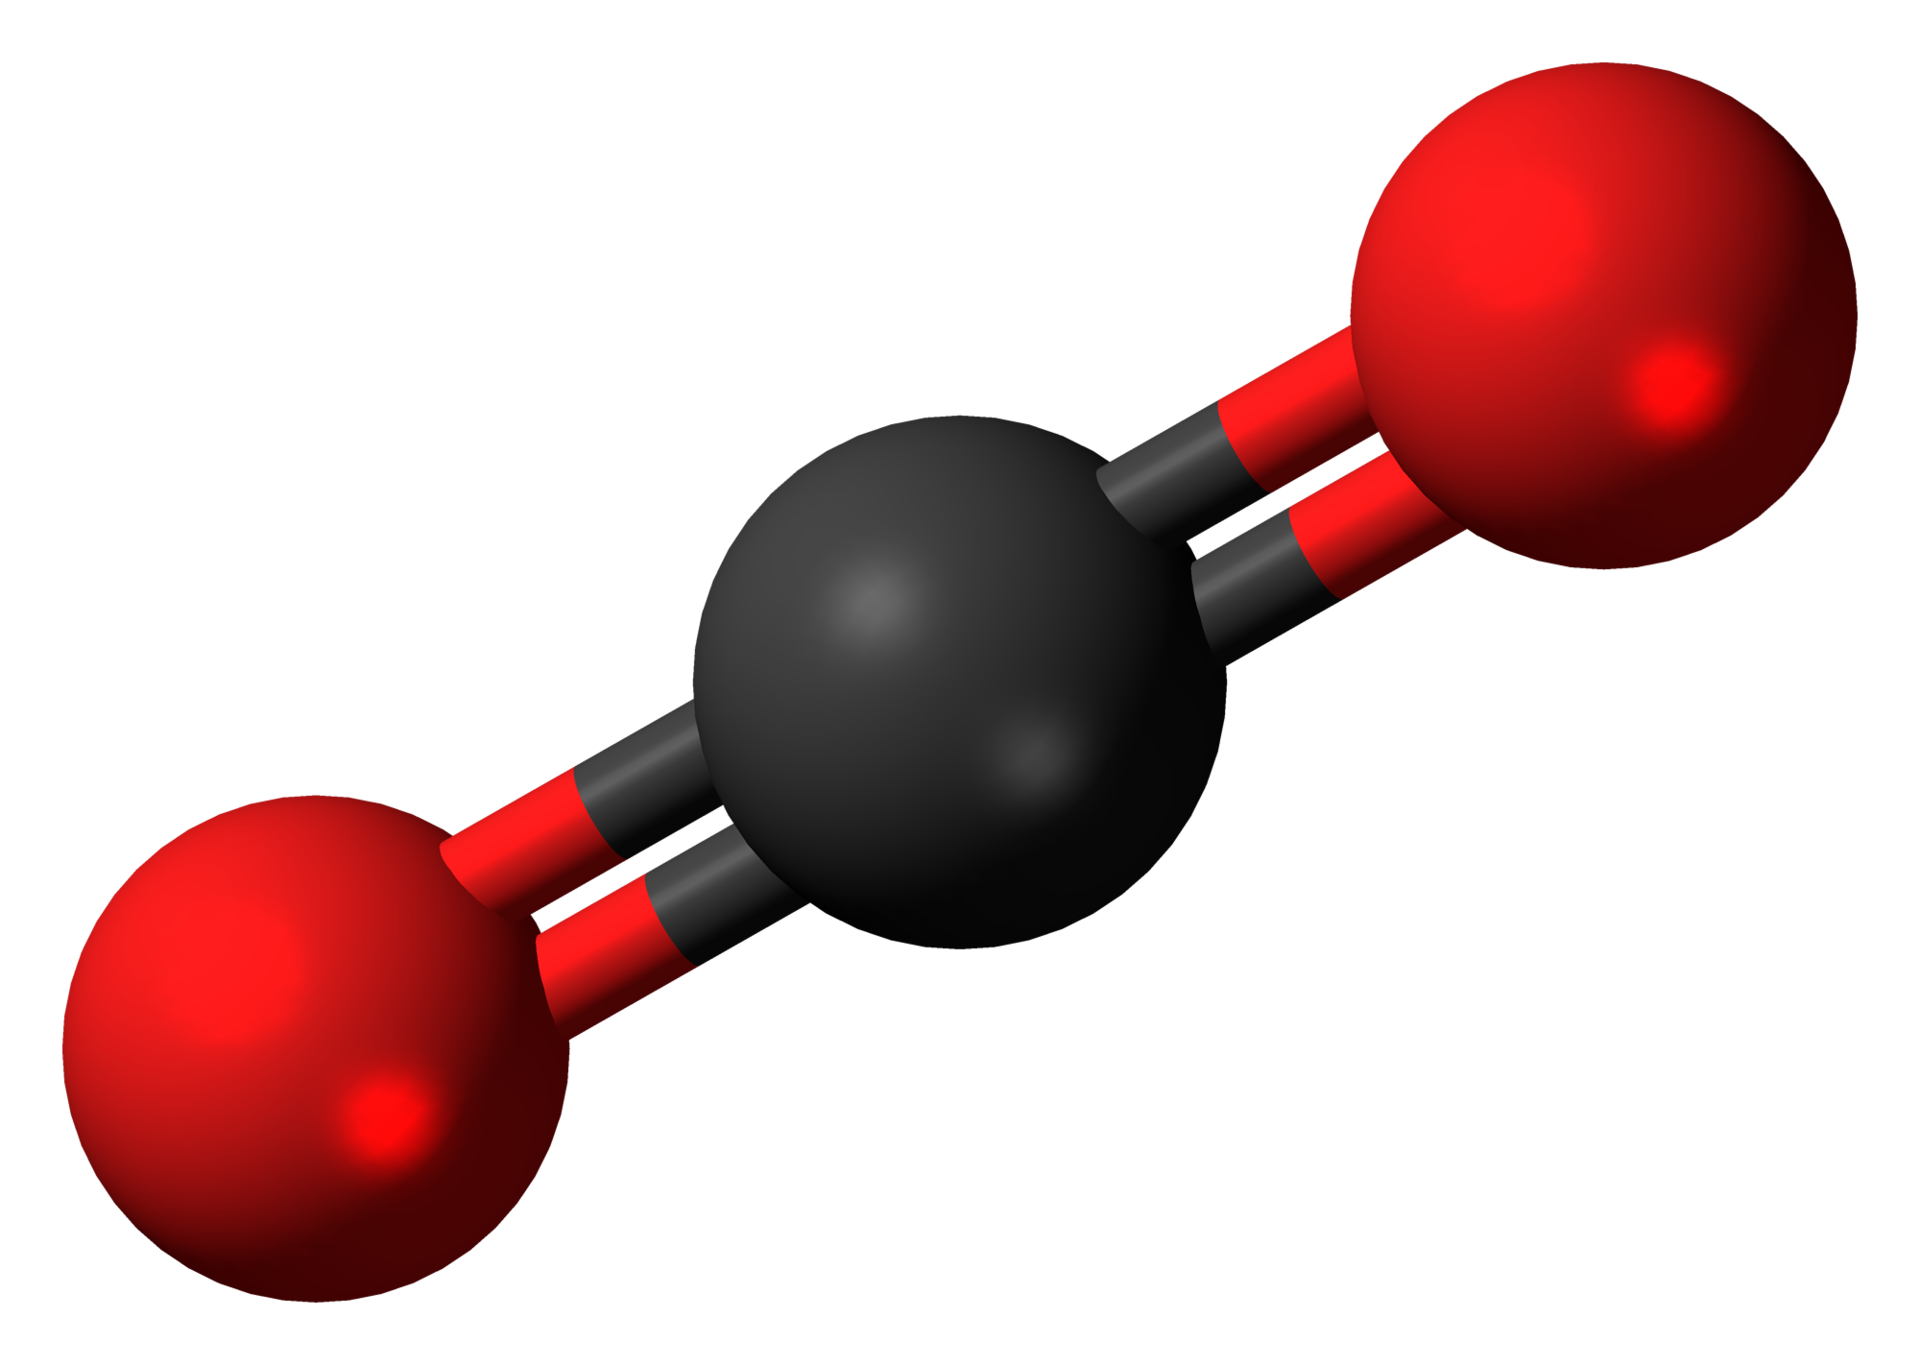
\includegraphics[width=0.25000\textwidth]{pictures/Carbon_dioxide_3D_ball.png}
\item
  Lewis dot structure:
  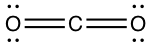
\includegraphics{pictures/CO2_lewis_structure.png}
\item
  Number of electron C has for itself following electronegativity rule:
  zero
\item
  \(CO_2\) can only be an electron acceptor
\item
  Production:

  \begin{itemize}
  \tightlist
  \item
    oxidation of C in all organic molecules
  \item
    Almost all respiratory processes on earth (some respiration does not
    involve oxidation of C)
  \item
    Combustion of all Carbon-based fuel
  \end{itemize}
\item
  Consumption:

  \begin{itemize}
  \tightlist
  \item
    Photosynthesis

    \begin{itemize}
    \tightlist
    \item
      Atmospheric carbon dioxide \textbf{is the primary carbon source
      for life} on Earth
    \end{itemize}
  \item
    Calcite precipitation in the oceans
  \end{itemize}
\item
  Ecological Significance:

  \begin{itemize}
  \tightlist
  \item
    Greenhouse Gas, which serves as reference for all other GHG
  \item
    Concentration in the atmosphere \textasciitilde{}380 ppm on the
    rise, or 0.38\%, or a partial pressure of 0.38 atm
  \end{itemize}
\end{itemize}

\begin{figure}
\centering
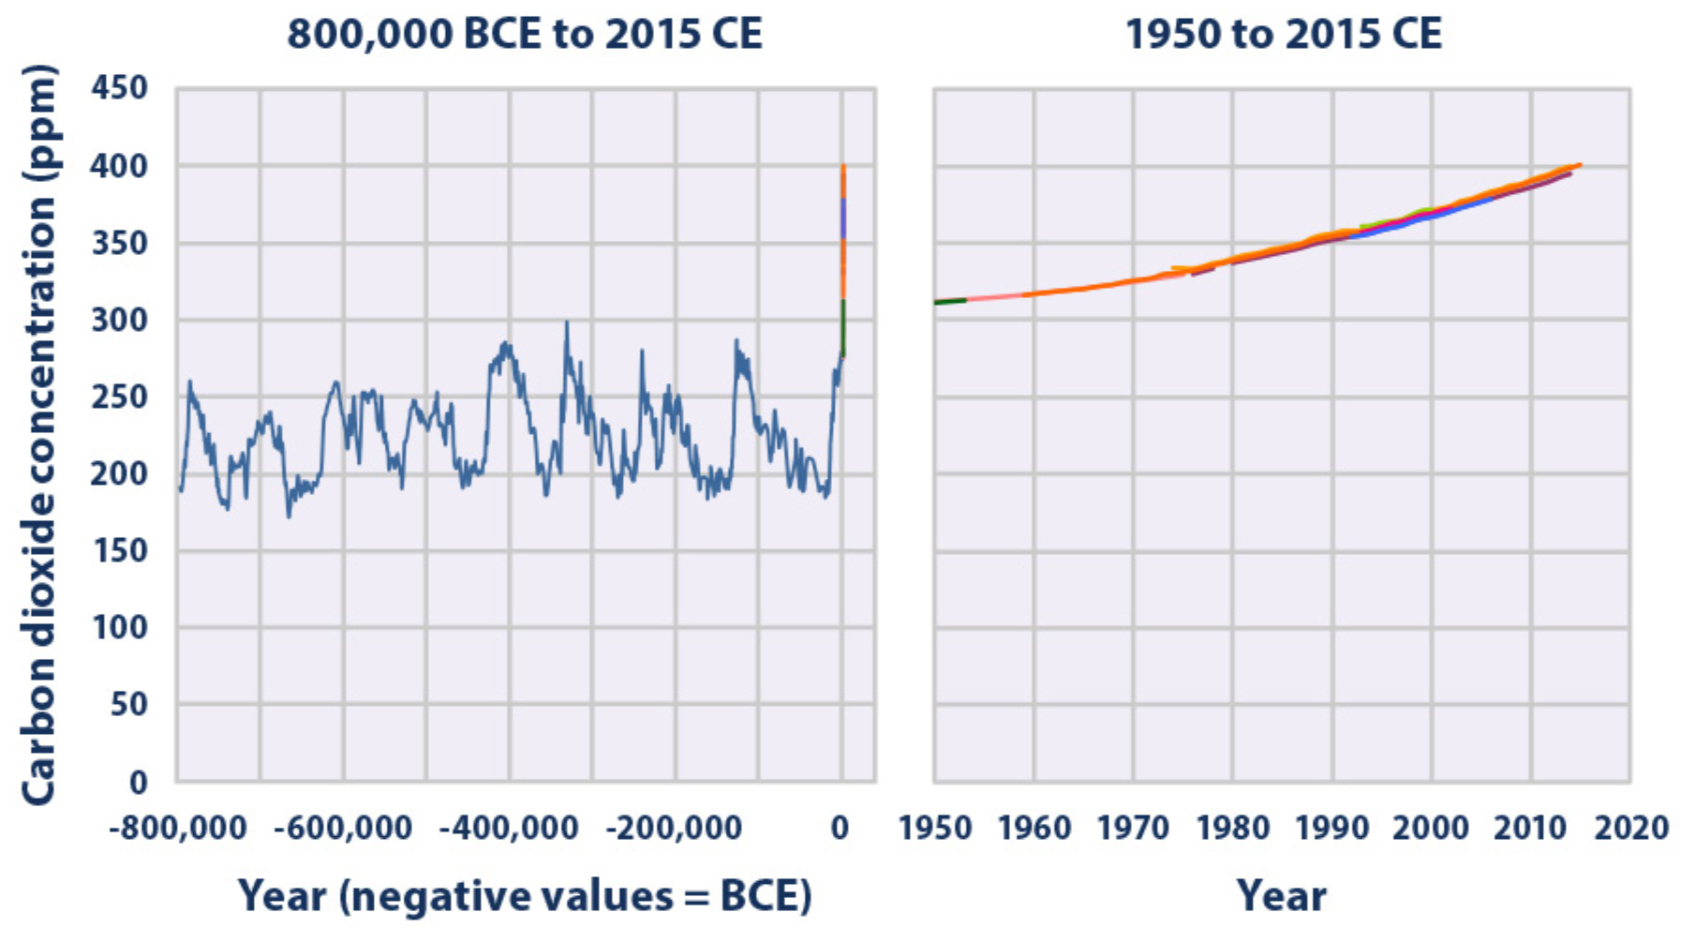
\includegraphics{pictures/CO2_atm_concentrations.png}
\caption{Carbon Dioxide variations through ancient and modern times}
\end{figure}

\href{https://https://www.epa.gov/sites/production/files/2016-08/documents/print_ghg-concentrations-2016.pdf}{concentrations
of carbon dioxide in the atmosphere from hundreds of thousands of years
ago through 2015, measured in parts per million (ppm). The data come
from a variety of historical ice core studies and recent air monitoring
sites around the world. Each line represents a different data source}

\begin{itemize}
\item
  In reality, concentrations are not stable, and vary widely in time and
  in space at the next two videos nicely show.
\item
  The next one results from the model simulations
\end{itemize}

\href{https://www.youtube.com/embed/WGHkY0E4FMY}{Youtube video of
\(CO_2\) modeled seasonal variations}

 - The following one is the combination of both models and observations

\href{https://www.youtube.com/embed/2BWWrJr6TJw}{Youtube video of
\(CO_2\) modeled and observed seasonal variations}

\emph{\protect\hyperlink{top}{back to top}}

\subsection{Carbonates}\label{carbonates}

\begin{itemize}
\tightlist
\item
  After carbon dioxide dissolves in water, it will combine with water to
  form carbonic acid (\(H_2CO_3\)).
\item
  Carbonate serves as \textbf{the carbon source} for aquatic vegetation
\item
  Carbonic acid can then dissociate into bicarbonate (\(HCO_3^-\)) and
  carbonate (\(CO_3^{2-}\))
\end{itemize}

\begin{align}
H_2CO_3  & \rightleftharpoons & HCO_3^- + H^+  \label{eq:H2CO3} \\
HCO_3^- & \rightleftharpoons & CO_3^{2-} + H^+ \label{eq:HCO3}
\end{align}

\texttt{\textbackslash{}tag\{\$pK\_A\$\ =\ 3.6\}}
\texttt{\textbackslash{}tag\{\$pK\_A\$\ =\ 6.35\}}

\begin{itemize}
\tightlist
\item
  In an environment not open to the atmosphere (or where direct exchange
  with the atmosphere is very limited like in stream or wetland
  sediment), the preponderant form depends on the pH and can be
  calculated as illustrated on the graph below.
\end{itemize}

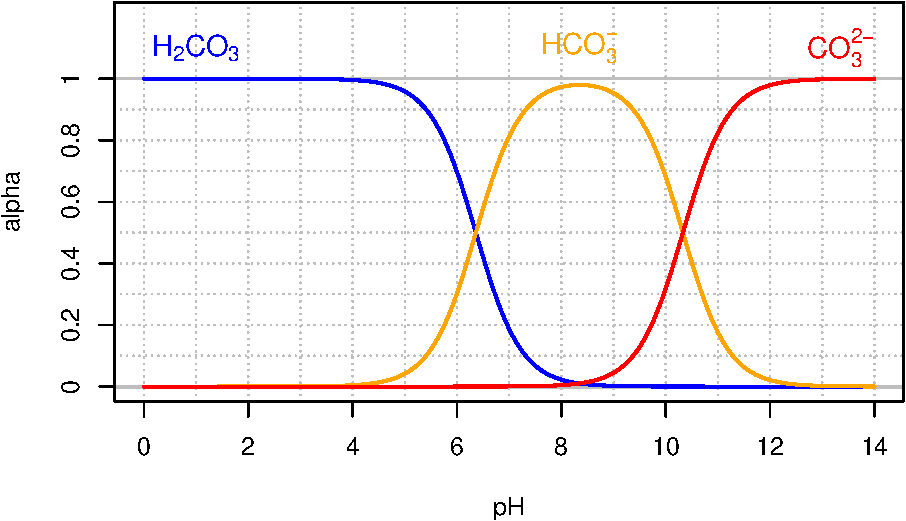
\includegraphics{bookdown-demo_files/figure-latex/CO3-1.pdf}

\begin{itemize}
\tightlist
\item
  In sea water, Carbonate can combine with \(Ca^{2+}\) to form Calcium
  Carbonate (\(CaCO_3\)), which precipitates out of solution. In other
  words, calcium carbonate formation is a sink for carbonate, and
  ultimately from \(CO_2\) addition from the atmosphere to to increased
  \(CO_2\) concentrations in the atmosphere.
\item
  Carbonates are thus a great pH buffer in aquatic environments
\end{itemize}

\section{D}\label{d}

\subsection{Dihydrogen sulfide}\label{dihydrogen-sulfide}

\begin{itemize}
\tightlist
\item
  see hydrogen sulfide
\end{itemize}

\emph{\protect\hyperlink{top}{back to top}}

\section{E}\label{e}

\hypertarget{eutrophication}{\subsection{Eutrophication}\label{eutrophication}}

\begin{itemize}
\tightlist
\item
  Definitions:

  \begin{itemize}
  \tightlist
  \item
    `an increase in the rate of supply of organic matter to an
    ecosystem' \citep{Nixon1995-th}
  \item
    `is the enrichment of a water body with nutrients, usually with an
    excess amount of nutrients' (Wikipedia)
  \item
    `the enrichment of water by nutrients, especially nitrogen and/or
    phosphorus, causing an accelerated growth of algae and higher forms
    of plant life to produce an undesirable disturbance to the balance
    of organisms present in the water and to the quality of water
    concerned' \citep{Anonymous1991-ho}
  \item
    `the enrichment of water by nitrogen compounds causing an
    accelerated growth of algae and higher forms of plant life to
    produce an undesirable disturbance to the balance of organisms
    present in the water and to the quality of water concerned'
    \citep{Anonymous1991-xb}
  \end{itemize}
\end{itemize}

\emph{\protect\hyperlink{top}{back to top}}

\section{G}\label{g}

\subsection{\texorpdfstring{Greenhouse gases
\emph{(GHG)}}{Greenhouse gases (GHG)}}\label{greenhouse-gases-ghg}

A greenhouse gas is a gas in an atmosphere that absorbs and emits
radiant energy within the thermal infrared range. This process is the
fundamental cause of the greenhouse effect. The primary greenhouse gases
in Earth's atmosphere are \textbf{water vapor},
\textbf{\protect\hyperlink{CO2}{carbon dioxide}}, \textbf{methane},
\textbf{\protect\hyperlink{N2O}{nitrous oxide}}, and \textbf{ozone}.
Without greenhouse gases, the average temperature of Earth's surface
would be about −18 °C (0 °F), rather than the present average of 15 °C
(59 °F). In the Solar System, the atmospheres of Venus, Mars and Titan
also contain gases that cause a greenhouse effect.
(\href{https://en.wikipedia.org/wiki/Greenhouse_gas}{Wikipedia})

\emph{\protect\hyperlink{top}{back to top}}

\section{H}\label{h}

\subsection{Haber-Bosch process}\label{haber-bosch-process}

\begin{itemize}
\tightlist
\item
  \href{https://en.wikipedia.org/wiki/Haber_process}{Haber-Bosch
  process}
\end{itemize}

\emph{\protect\hyperlink{top}{back to top}}

\subsection{Hydrogen Sulfide}\label{hydrogen-sulfide}

\begin{itemize}
\tightlist
\item
  It is a colorless gas with the characteristic foul odor of rotten
  eggs.
\item
  It is very poisonous, corrosive, flammable and acidic in nature.
\item
  Formula: \(H_2S\)
\item
  hydrogen sulfide \#D shape:
  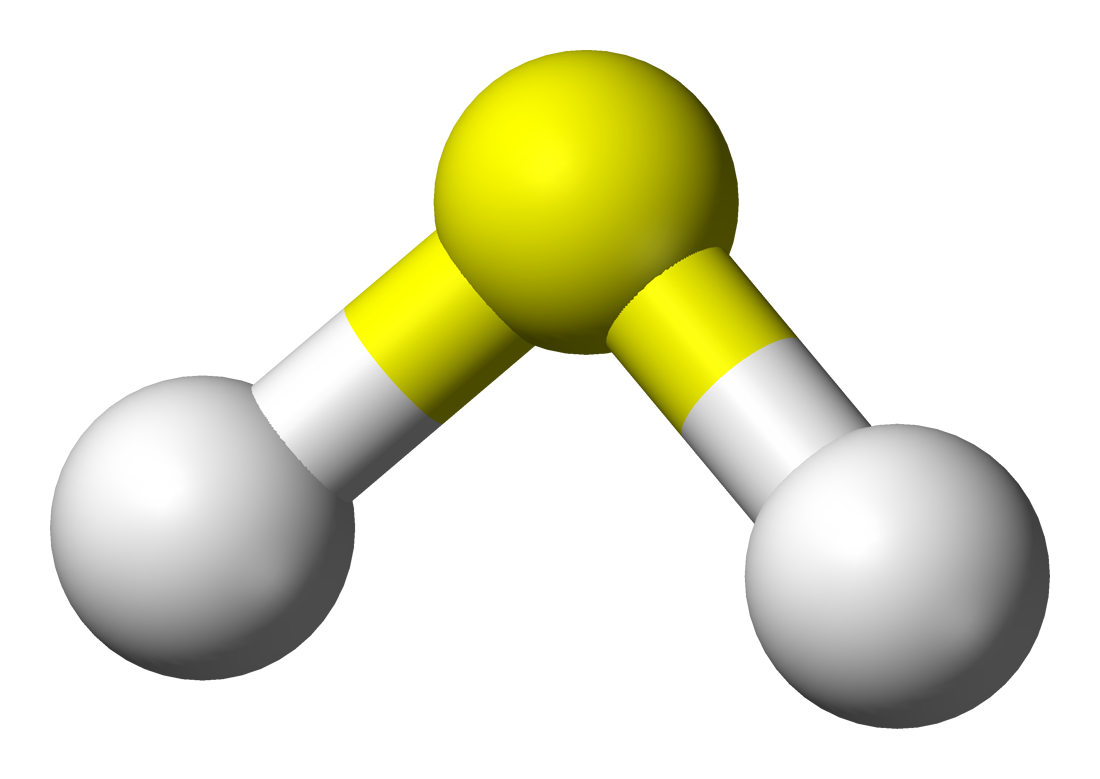
\includegraphics[width=0.25000\textwidth]{pictures/Hydrogen-sulfide-3D-balls.png}
\item
  Lewis dot structure:
  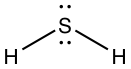
\includegraphics[width=0.25000\textwidth]{pictures/H2S_Lewis_structure.png}
\item
  Number of electron S has for itself following electronegativity rule:
  eight
\item
  \(H_2S\) can only be an electron donor
\item
  Unstable under aerobic conditions, will readily be oxidized into
  \protect\hyperlink{SO4}{sulfate}
\item
  \(H_2S\) is a polyprotic acid which can lose up to 2 protons in water,
  depending on the pH.
\end{itemize}

\begin{align}
H_2S & \rightleftharpoons & HS^- + H^+ \label{eq:H2S} \\
HS^- & \rightleftharpoons & S^{2-}+ H^+ \label{eq:HS} 
\end{align}

\begin{itemize}
\tightlist
\item
  The figure below suggests that at pH found in most streams (4.5 to 8),
  \(H_2S\) is either preponderant or corresponds to at least 20\% of all
  sulfide forms. \(H_2S\) being a highly volatile product, it explains
  why we can easily smell and detect it in most conditions in streams.
\end{itemize}

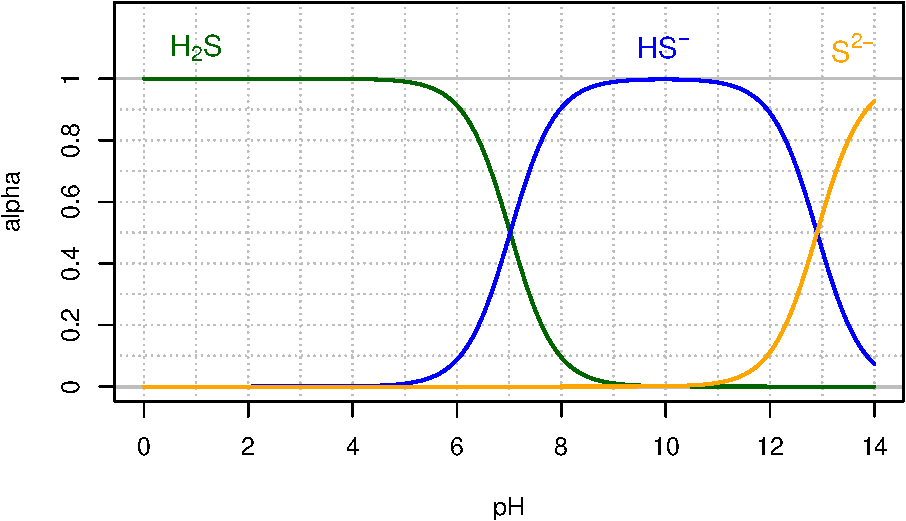
\includegraphics{bookdown-demo_files/figure-latex/H2S-1.pdf}

\begin{itemize}
\tightlist
\item
  Production:

  \begin{itemize}
  \tightlist
  \item
    Hydrogen sulfide often results from the microbial breakdown, or
    mineralization, of organic matter in anaerobic conditions, such as
    may exist in swamps and sewers. When happening in sediment, this is
    referred to as sediment diagenesis
  \end{itemize}
\item
  Consumption:
\end{itemize}

\emph{\protect\hyperlink{top}{back to top}}

\section{L}\label{l}

\subsection{Limiting factor}\label{limiting-factor}

\emph{\protect\hyperlink{top}{back to top}}

\section{M}\label{m}

\subsection{Methane}\label{methane}

\begin{itemize}
\tightlist
\item
  Under
  \href{https://en.wikipedia.org/wiki/Standard_conditions_for_temperature_and_pressure}{normal
  conditions for temperature and pressure}, methane is a colorless,
  odorless gas main constituent of natural gas, and the simplest alkane
\item
  Formula: \(CH_4\)
\item
  Methane 3D shape:
  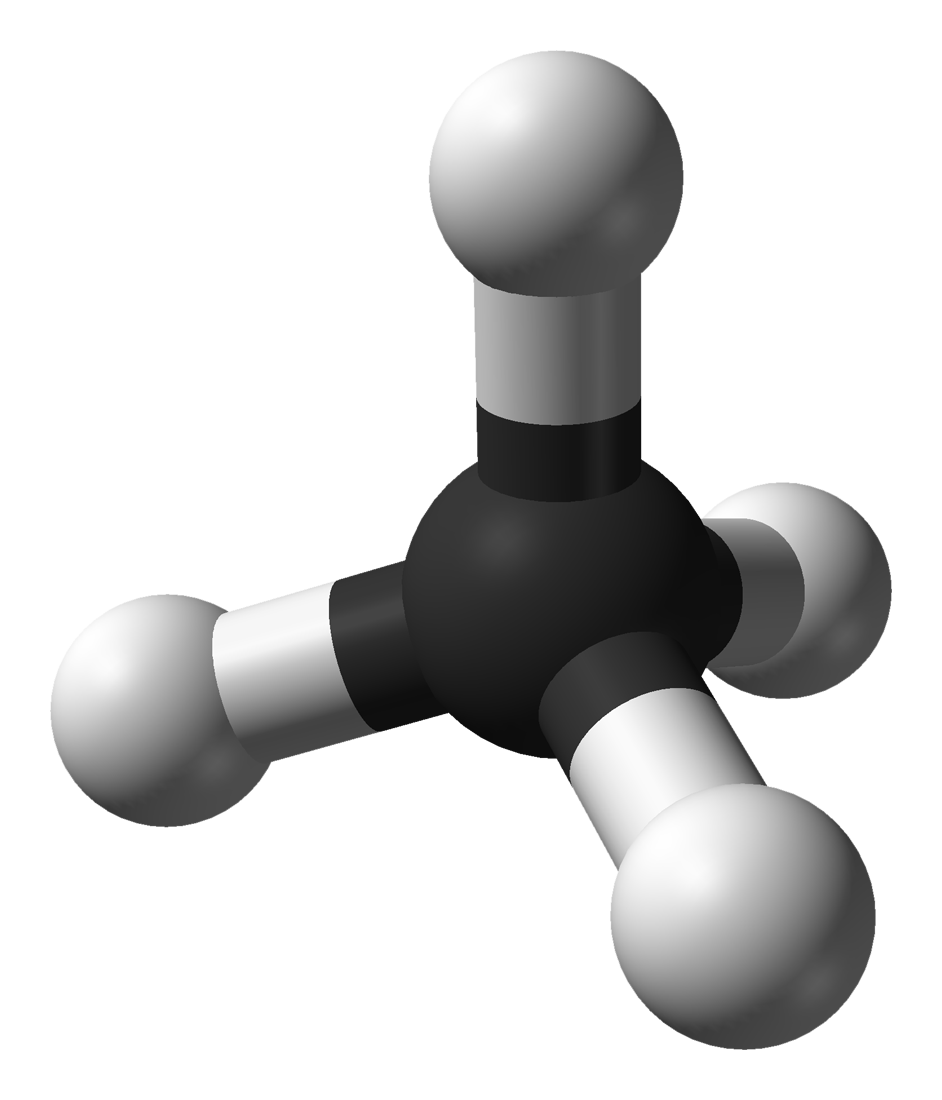
\includegraphics[width=0.25000\textwidth]{pictures/Methane-CRC-MW-3D-balls.png}
\item
  Lewis dot structure of methane:
  \includegraphics{pictures/methane_lewis_structure.png}
\item
  Number of electron C has for itself following electronegativity rule:
  eight
\item
  \(CH_4\) can only be an electron \textbf{donor}
\item
  Because methane has so many electrons to give, it will easily `burn'
  in normal atmosphere (provided that ignition T°C be reached, e.g., by
  a spark), liberating large quantities of heat (55.5 MJ/kg). The
  electrons are transferred from the carbon to the oxygen atoms
  following two redox half-reactions to obtain the overall reaction:
\end{itemize}

\begin{align}
CH_4 + 2\,H_2O & \rightleftharpoons & CO_2 + 8\,H^+ + 8\,e^-\\
2\,O_2 + 8\,H^+ + 8\,e^- & \rightleftharpoons & 4\,H_2O\\
& &\\
\hline\\
CH_4 + 2\,O_2 & \to & CO_2 + 2\,H_2O
\end{align}

\begin{itemize}
\item
  Production:
\item
  Consumption:
\item
  Ecological significance:
\end{itemize}

\begin{figure}
\centering
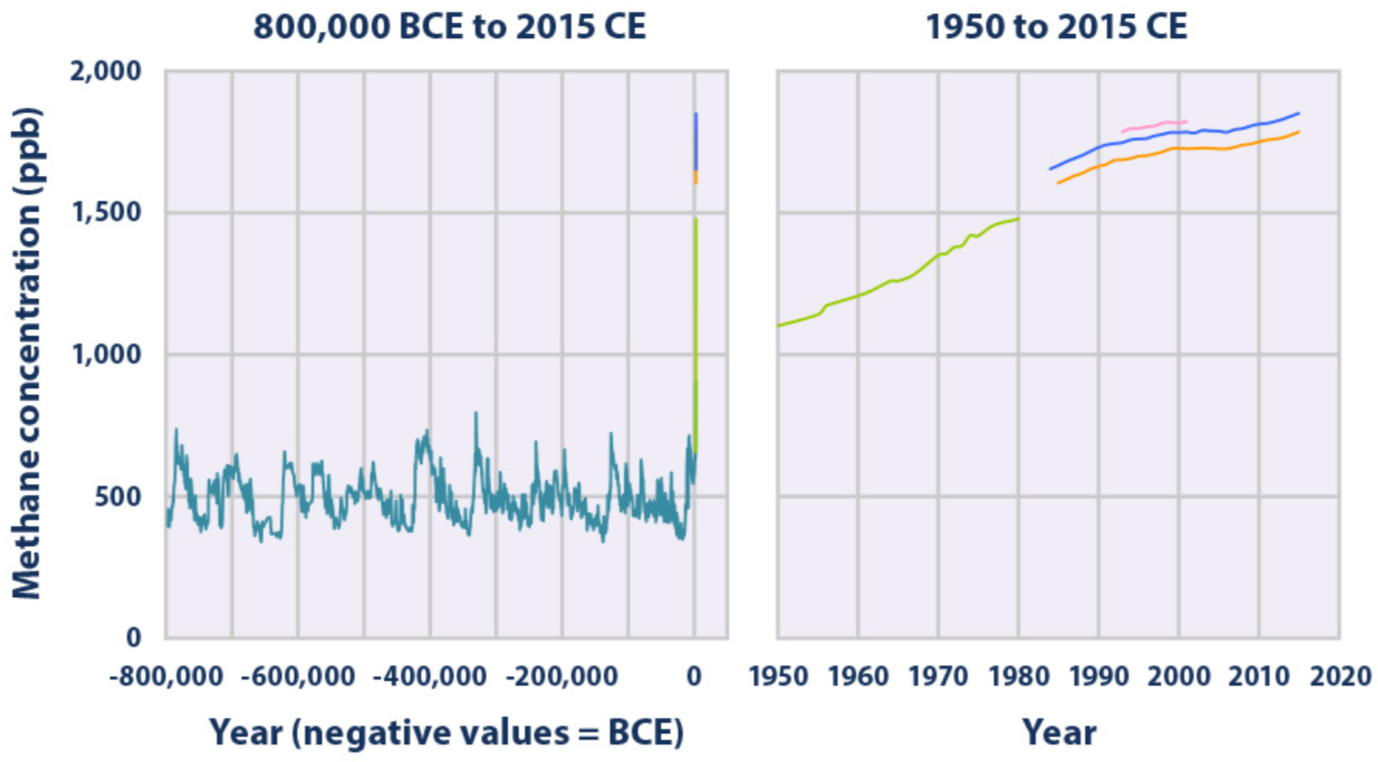
\includegraphics{pictures/CH4_concentrations.png}
\caption{}
\end{figure}

\href{https://www.epa.gov/sites/production/files/2016-08/documents/print_ghg-concentrations-2016.pdf}{Concentrations
of methane in the atmosphere from hundreds of thousands of years ago
through 2015, measured in parts per billion (ppb). The data come from a
variety of historical ice core studies and recent air monitoring sites
around the world. Each line represents a different data source}

\begin{itemize}
\tightlist
\item
  Health effects:
\end{itemize}

\section{N}\label{n}

\subsection{Nitrate}\label{nitrate}

\begin{itemize}
\item
  Nitrate is the stable inorganic nitrogenous anion in oxidized water
\item
  Formula: \(NO_3^{-}\)
\item
  Nitrate 3D shape:
  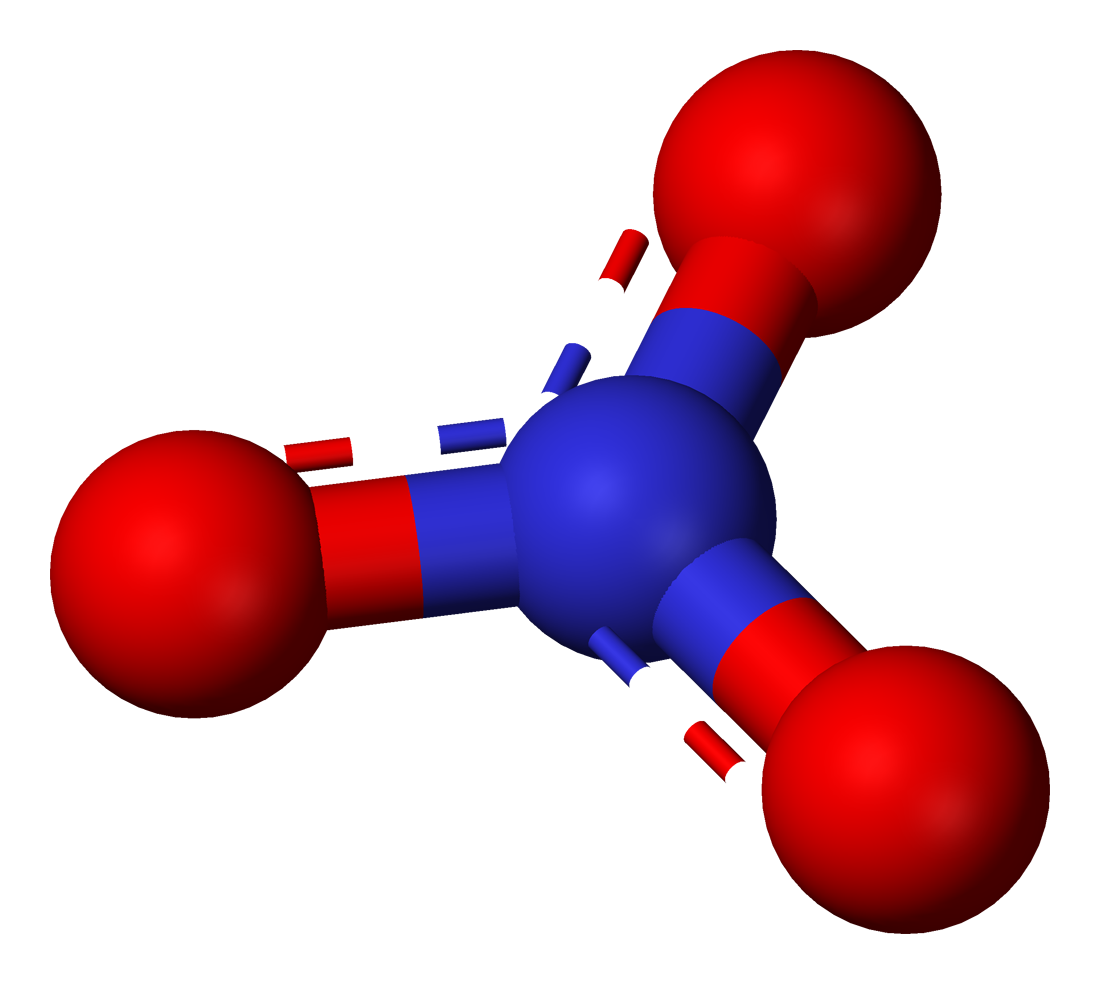
\includegraphics[width=0.25000\textwidth]{pictures/Nitrate-3D-balls.png}
\item
  Lewis dot structure of nitrate:
  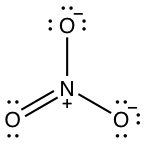
\includegraphics{pictures/nitrate_lewis_structure.png}
\item
  Number of electron N has for itself following electronegativity rule:
  zero
\item
  \(NO_3^{-}\) can only be an electron acceptor
\item
  \(NO_3^{-}\) is technically the conjugate base of nitric acid
  \(HNO_3\), but the \(pk_A\) of the reaction is at a theoretical pH of
  -1.38. In other words, for the pH of most natural waters (4.5
  \textless{} pH \textless{} 8), \(HNO_3\) is totally insignificant.
\item
  Production:

  \begin{itemize}
  \tightlist
  \item
    from the complete \protect\hyperlink{oxidation}{oxidation} of
    inorganic nitrogenous molecules which include
    \protect\hyperlink{NH3}{ammonia}, \protect\hyperlink{NH4}{ammonium},
    \protect\hyperlink{NO2}{nitrite}
  \item
    from the mineralization and complete oxidation of
    \protect\hyperlink{amine}{amine radicals} in organic molecules
  \end{itemize}
\item
  Consumption:

  \begin{itemize}
  \tightlist
  \item
    \textbf{Uptake} from microbes, plants, and algae for their
    \protect\hyperlink{anabolism}{anabolism}, which consists in building
    complex organic molecules from inorganic ones.

    \begin{itemize}
    \tightlist
    \item
      Uptake, assimilation, anabolism, immobilization are all synonymous
      terms to express the fact that the N atom is immobilized, at least
      temporarily in organic molecules.
    \item
      Because N is assimilated in organic molecules during
      uptake/anabolism, and because N gains electrons in the process (it
      is thus \textbf{\emph{reduced}}), we refer to nitrate uptake as
      \textbf{\protect\hyperlink{ANR}{assimilatory nitrate reduction}}.
    \end{itemize}
  \item
    \textbf{\protect\hyperlink{denitrification}{Denitrification}}: under
    anaerobic conditions, nitrate is used by facultative anaerobes as
    electron acceptor to generate \protect\hyperlink{ATP}{ATP} in their
    respiration chain. The two major end products of denitrification are
    gases, namely \protect\hyperlink{N2}{dinitrogen (\(N_2\))} and
    \protect\hyperlink{N2O}{nitrous oxide (\(N_2O\))}, which leave the
    aqueous environment. As such, nitrate is not assimilated by any
    bacteria and denitrification is therefore, as opposed to uptake,
    referred to as **\protect\hyperlink{DNR}{dissimilatory nitrate
    reduction} into \protect\hyperlink{N2}{dinitrogen (\(N_2\))} and
    \protect\hyperlink{N2O}{nitrous oxide (\(N_2O\))}.
  \end{itemize}
\item
  Ecological significance:

  \begin{itemize}
  \tightlist
  \item
    Because of assimilation and denitrification processes, the overall
    nitrate concentrations in rivers tends to diminish from the
    catchment headwaters to the receiving bodies such as estuaries and
    coastal areas. As a result, inorganic nitrogen has naturally been in
    very short supply in these coastal water bodies, and nitrate and
    traditionally been the nutrient limiting aquatic productivity there.
    Very much like with phosphate, algae have adapted to be able to grow
    in very low concentrations. Anthropogenic activities, and
    agriculture in particular, have largely increased the loads and
    concentration of nitrate reaching estuaries, to the point where
    nitrate is no longer the limiting factor. As a result, excess
    nitrate is one of the reasons for the global and persistent presence
    of algal blooms in estuaries and coastal waters.
  \end{itemize}
\item
  Health hazard:

  \begin{itemize}
  \tightlist
  \item
    There is a heated debate about the health hazard that nitrate might
    pose. Some argue that if anything, there might be beneficial
    effects, while others argue that there are evidence of cancers
    linked to excess nitrate absorption. Unfortunately, arguments on
    both sides might not be totally independent of militantism and
    lobbies.
  \item
    The only consensus everybody seems to agree upon is the Blue Baby
    syndrome, or methemoglobinemia. Methemoglobinemia is an unusual and
    potentially fatal condition in which hemoglobin is oxidized to
    methemoglobin and loses its ability to bind and transport oxygen,
    hence the cyanosis (blue appearance) usually visible on fingers,
    toes, and lips. Nitrate reduced to nitrite in the body of humans and
    animals enters the body stream where it seems to directly oxidize
    oxyhemoglobin to methemoglobin-peroxide complex.
  \end{itemize}
\end{itemize}

\href{https://syndromespedia.com/blue-baby-syndrome.html}{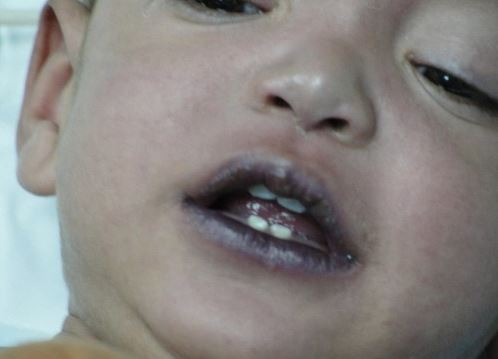
\includegraphics[width=0.50000\textwidth]{pictures/BLUE-BABY-SYNDROME.jpg}}

\href{https://syndromespedia.com/blue-baby-syndrome.html}{\textbf{Picture
of a Blue Baby from syndromespedia.com/blue-baby-syndrome.html}}

\begin{itemize}
\tightlist
\item
  Drinking water standards

  \begin{itemize}
  \tightlist
  \item
    Although there is still a heated debate whether or not nitrate does
    have have detrimental health effects, the World Health Organization
    has provided maximum concentration guidelines of 50 mg/L as nitrate
    \citep{World_Health_Organization2011-hd}. These guidelines have been
    enacted in hard laws in the US and in Europe. The 50 mg/L as nitrate
    equates 11.2 mg \(NO_3\)-N/L and in the US, the drinking water
    standard is \textbf{10 mg \(NO_3\)-N/L}.
  \end{itemize}
\end{itemize}

\emph{\protect\hyperlink{top}{back to top}}

\subsection{Nitrous Oxide}\label{nitrous-oxide}

\begin{itemize}
\item
  Commonly known as laughing gas
\item
  Nitrous oxide has significant medical uses, especially in surgery and
  dentistry, for its anesthetic and pain reducing effects.
\item
  Formula: \(N_2O\)
\item
  Nitrous Oxide 3D shape:
  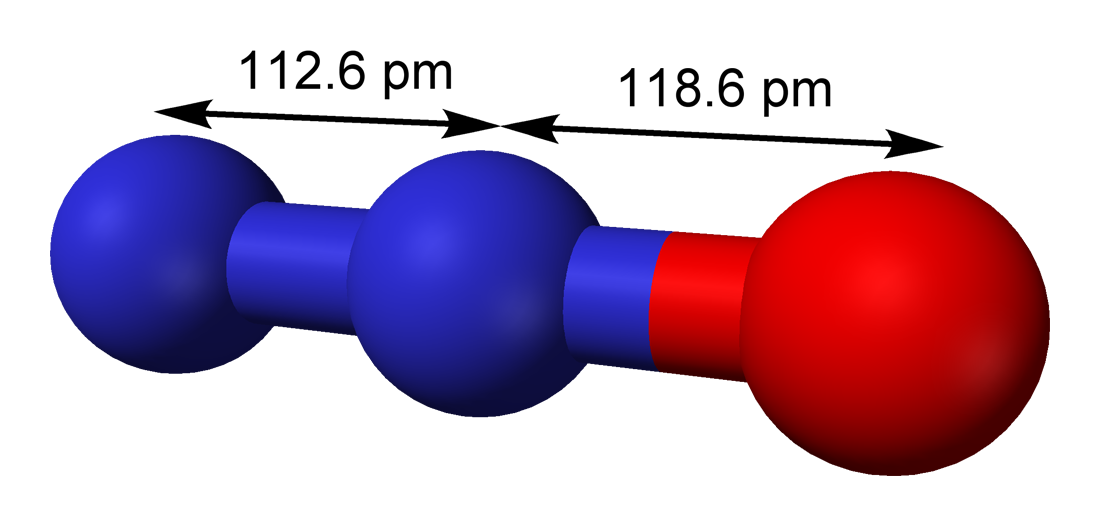
\includegraphics[width=0.25000\textwidth]{pictures/Nitrous-oxide-dimensions-3D-balls.png}
\item
  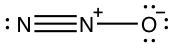
\includegraphics[width=0.25000\textwidth]{pictures/N2O_lewis_structure.png}
\item
  Number of electron N has for itself following electronegativity rule:

  \begin{itemize}
  \tightlist
  \item
    the first one on the left has 5
  \item
    the middle N has 3
  \end{itemize}
\item
  \(N_2O\) can be both an electron acceptor and an electron donor
\item
  Production:

  \begin{itemize}
  \tightlist
  \item
    \(N_2O\) is produced due to bacterial processes (over 90\%) and
    anthropogenic processes such as burning of fossil fuel

    \begin{itemize}
    \tightlist
    \item
      The two main bacterial processes are \emph{nitrification} and
      \emph{denitrification}
    \item
      Accounting that human activities have enhanced both nitrification
      and denitrification processes, it is estimated that overall, about
      2/3rd of \(N_2O\) production is natural, and about 1/3rd is human
      enhanced
    \end{itemize}
  \end{itemize}
\item
  Consumption:

  \begin{itemize}
  \tightlist
  \item
    Because of all the electrons stored on the two N atoms (5 + 3 = 8),
    nitrous oxide is a potential electron donor and bacteria can use it
    for their respiration processes
  \end{itemize}
\item
  Ecological significance:
\item
  Powerful Greenhouse Gas, 298 times that of \(CO_2\)
  (\href{https://www.epa.gov/sites/production/files/2015-07/documents/emission-factors_2014.pdf}{EPA})
\item
  Concentration in the atmosphere \textasciitilde{}0.0003 ppm or
  \textasciitilde{}325 ppb on the rise
\end{itemize}

\begin{figure}
\centering
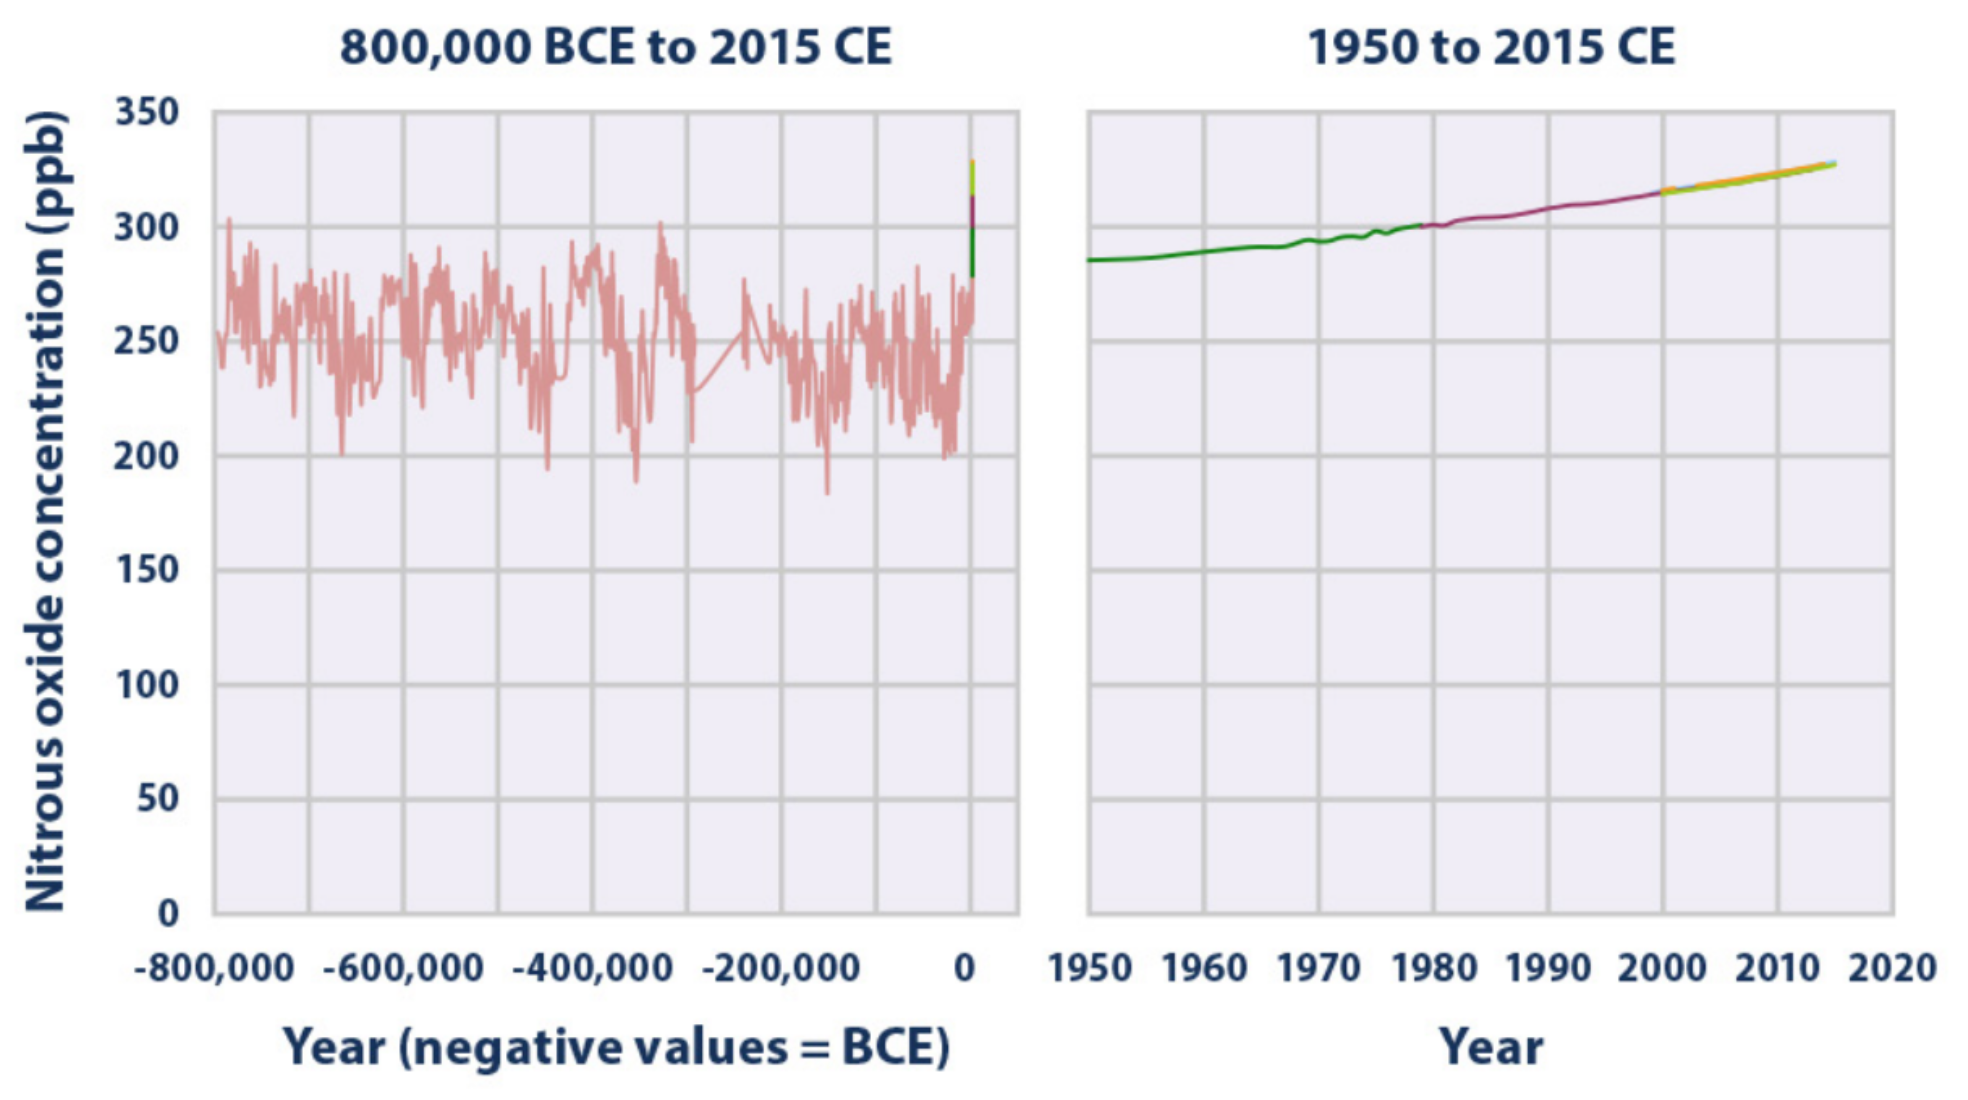
\includegraphics{pictures/N2O_concentrations.png}
\caption{}
\end{figure}

\href{https://www.epa.gov/sites/production/files/2016-08/documents/print_ghg-concentrations-2016.pdf}{Concentrations
of nitrous oxide in the atmosphere from hundreds of thousands of years
ago through 2015, measured in parts per billion (ppb). The data come
from a variety of historical ice core studies and recent air monitoring
sites around the world. Each line represents a different data source})

\emph{\protect\hyperlink{top}{back to top}}

\section{O}\label{o}

\subsection{Oligotrophication}\label{oligotrophication}

\begin{itemize}
\tightlist
\item
  `a decrease in the rate of supply of organic matter to an ecosystem'
  \citep{Nixon2009-ft}
\end{itemize}

\emph{\protect\hyperlink{top}{back to top}}

\section{P}\label{p}

\subsection{Phosphate}\label{phosphate}

\begin{itemize}
\tightlist
\item
  \href{https://en.wikipedia.org/wiki/Phosphate}{Phosphate} is an
  inorganic chemical and a salt-forming anion of phosphoric acid
\item
  Formula: \(PO_4^{3-}\)
\item
  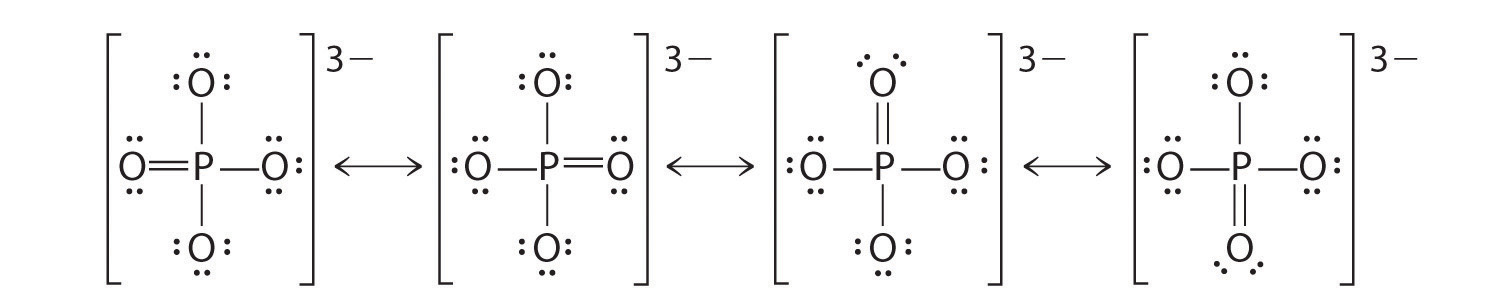
\includegraphics{pictures/phosphate_lewis_structure.jpg}
\item
  Phosphate is one of the anions of the polyprotic acid (i.e., which can
  liberate several protons \(H^{+}\))
\item
  The conjugate bases of phosphate are:
  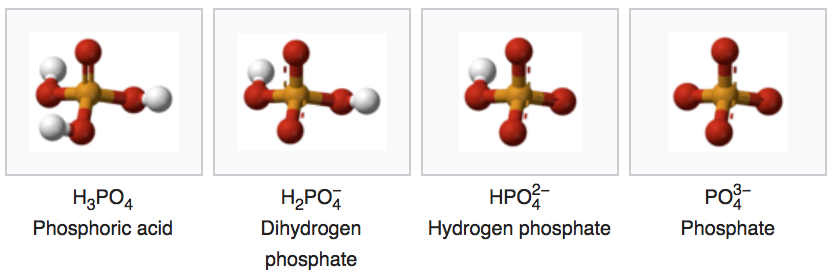
\includegraphics[width=1.00000\textwidth]{pictures/phosphate_conjugate_bases.png}
\item
  All conjugate bases are related through the set acid-base chemical
  equilibria:
\end{itemize}

\begin{align}
H_3PO_4  & \rightleftharpoons & H_2PO_4^- + H^+ \tag{$pK_A$ = 2.12}\\
H_2PO_4^- & \rightleftharpoons & HPO_4^{2-} + H^+ \tag{$pK_A$ = 7.21}\\
HPO_4^{2-}& \rightleftharpoons & PO_4^{3-} + H^+ \tag{$pK_A$ = 12.67}
\end{align}

\begin{itemize}
\tightlist
\item
  The preponderant form of phosphate in a solution also depends on the
  pH following this relationship:
\end{itemize}

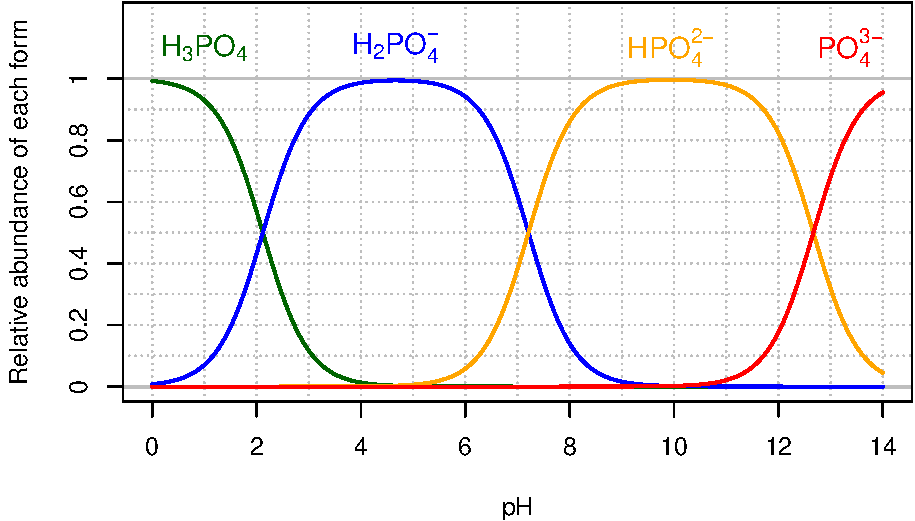
\includegraphics{bookdown-demo_files/figure-latex/phosphates-1.pdf}

\begin{itemize}
\tightlist
\item
  Production:

  \begin{itemize}
  \tightlist
  \item
    Phosphorus in general and phosphate in practice has remained one of
    the nutrients limiting the most plant productivity on our planet
  \item
    Phosphates are the naturally occurring form of the element
    phosphorus, found in many phosphate minerals
  \item
    Phosphate minerals are mined to obtain phosphorus for use in
    agriculture and industry
  \item
    The largest global producer and exporter of phosphates is Morocco.
  \item
    Within North America, the largest deposits lie in the Bone Valley
    region of central Florida, the Soda Springs region of southeastern
    Idaho, and the coast of North Carolina (near Aurora).
  \end{itemize}
\item
  Consumption:

  \begin{itemize}
  \tightlist
  \item
    Uptake from all primary producer including plants and algae
  \item
    Phosphate can also be immobilized by bacteria
  \item
    In food industry, phosphates help baked goods rise, they act as
    emulsifiers in processed cheese and canned soup, they add flavor to
    cola and color to frozen french fries. They also can be added to
    meat, poultry and seafood to help the protein bind more water,
    making it juicier after freezing and reheating.
  \end{itemize}
\item
  Ecological significance:

  \begin{itemize}
  \tightlist
  \item
    Phosphorus as phosphate naturally is the most limiting factor for
    primary productivity for land and aquatic plants. Because it tends
    to bind to particles, phosphates have accumulated with sediment
    particularly in coastal areas, where phosphate can become available
    again to algae through
    \protect\hyperlink{sediment_diagenesis}{sediment diagenetic
    processes}. As a result, phosphate is generally not considered the
    most limiting factor for algae in estuaries and coastal environment.
    However, it does tend to be the limiting nutrient in freshwater
    receiving bodies such as lakes and reservoirs.
  \item
    Excess phosphate in freshwater receiving bodies has been shown to be
    the nutrient causing some major
    \protect\hyperlink{eutrophication}{eutrophication} problems
    throughout the planet
  \end{itemize}
\end{itemize}

\emph{\protect\hyperlink{top}{back to top}}

\section{S}\label{s}

\subsection{Sulfate}\label{sulfate}

\begin{itemize}
\tightlist
\item
  Sulfate is the inorganic sulfur anion stable in oxidized water
\item
  Formula: \(SO_4^{2-}\)
\item
  Sulfate 3D shape:
  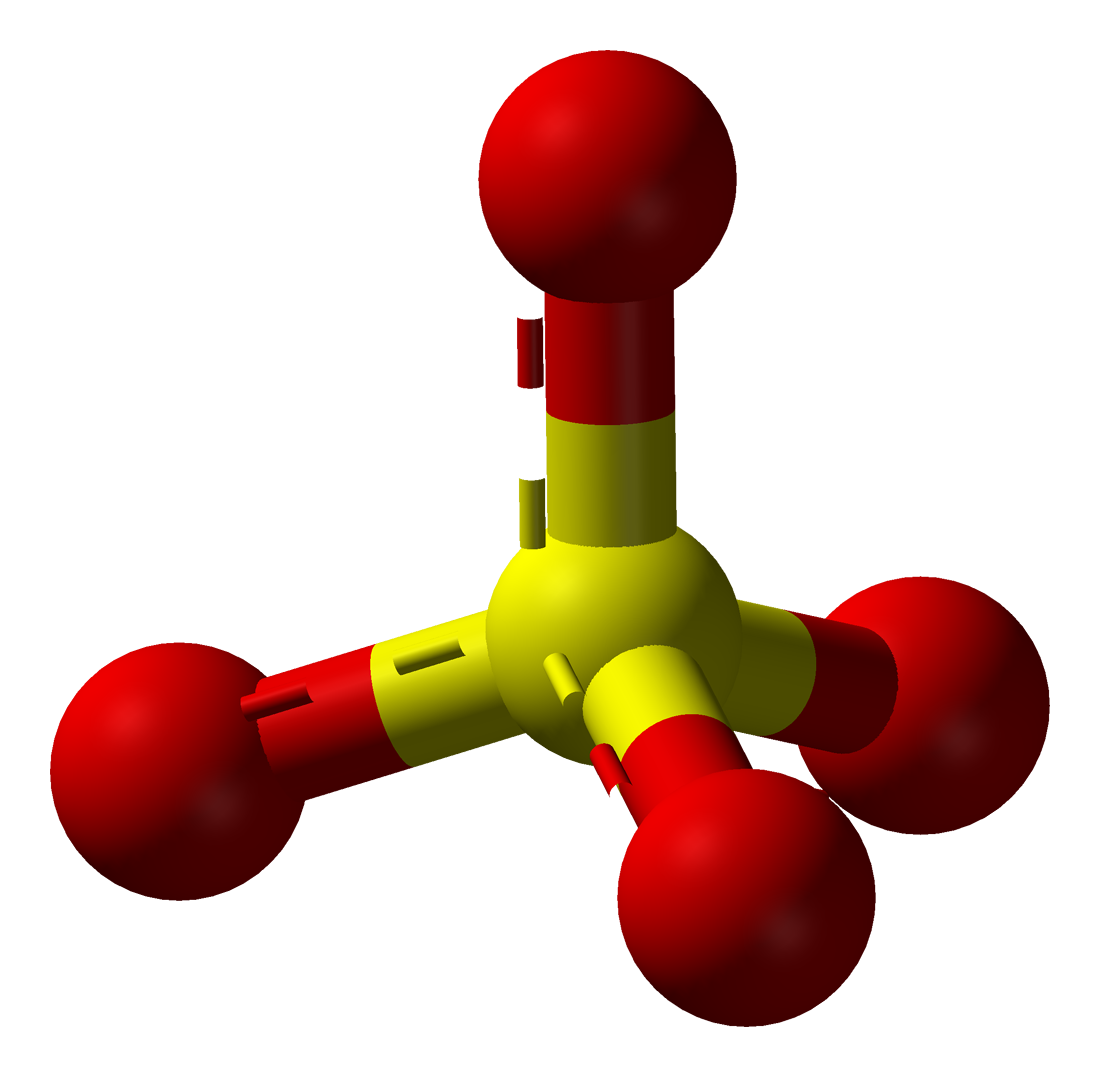
\includegraphics[width=0.25000\textwidth]{pictures/Sulfate-3D-balls.png}
\item
  Lewis dot structure of nitrate:
  \includegraphics{pictures/sulfate_lewis_structure.png}
\item
  Number of electron S has for itself following electronegativity rule:
  zero
\item
  \(SO_4^{2-}\) can only be an \emph{\textbf{electron acceptor}}
\item
  \(SO_4^{2-}\) is the conjugate base of Hydrogen sulfate \(HSO_4^{-}\).
  The figure below shows that for pH normally measured in surface water
  and streams (4.5-8), \(SO_4^{2-}\) is the truly preponderant form. We
  therefore generally omit to mention \(HSO_4^{-}\) as a chemical form
  that plays any significant role.
\end{itemize}

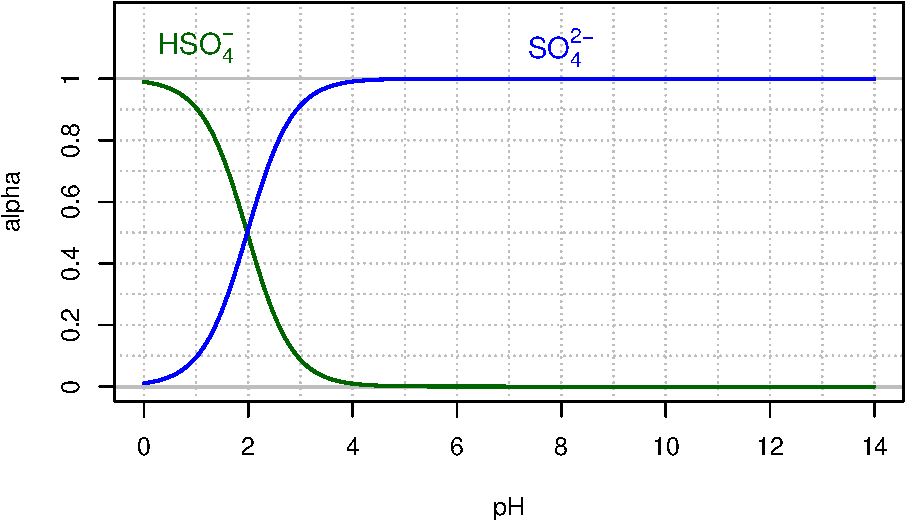
\includegraphics{bookdown-demo_files/figure-latex/SO4-1.pdf}

\begin{itemize}
\item
  During their anabolism, primary producers uptake sulfate, but the
  sulfur atoms can be incorporated into amino-acids only after sulfur
  has been reduced, or gained 8 electrons to be in a thiol (\(-SH\))
  form.
\item
  Production:
\item
  Consumption:
\item
  Ecological significance:
\item
  Health effects:
\end{itemize}

\emph{\protect\hyperlink{top}{back to top}}

\bibliography{book.bib,packages.bib}


\end{document}
